
\section{Experiment setup}
In this section we will be presenting the results regarding the different experiments performed over the datasets using the methods previously introduced. All the experiments will have different sets of requirements and levels of complexity, what will help us discern the capabilities of the tools involved. To be able to do so, we have to establish the same structured tests on every dataset\footnote{Due to the impossibility of using \texttt{caret::train} on MNIST (Every laptop I tried to use for this purpose would just get stuck and force the closing of RStudio), we will be not be using Knn to compare results on PCA and the Autoencoder. }.

We retake here the training scheme introduced in Chapter~\ref{chap:Introduction} and presented in Figure~\ref{fig:fig1}.\subref{fig:fig1a} where the \emph{first} half of the Autoencoder, the actual encoder, is used as a mechanism to obtain an efficient representation $\hat Z$ of the input data $\hat X$. 
%
We will use this representation  as the input for the classifier. 
%
In the following we use both a KNN and a MLP classifiers, as depicted in Figure~\ref{fig:Autoencoder_architecture}. 
%
\begin{figure}[H]
\begin{subfigure}{1\linewidth}  
 \centering
  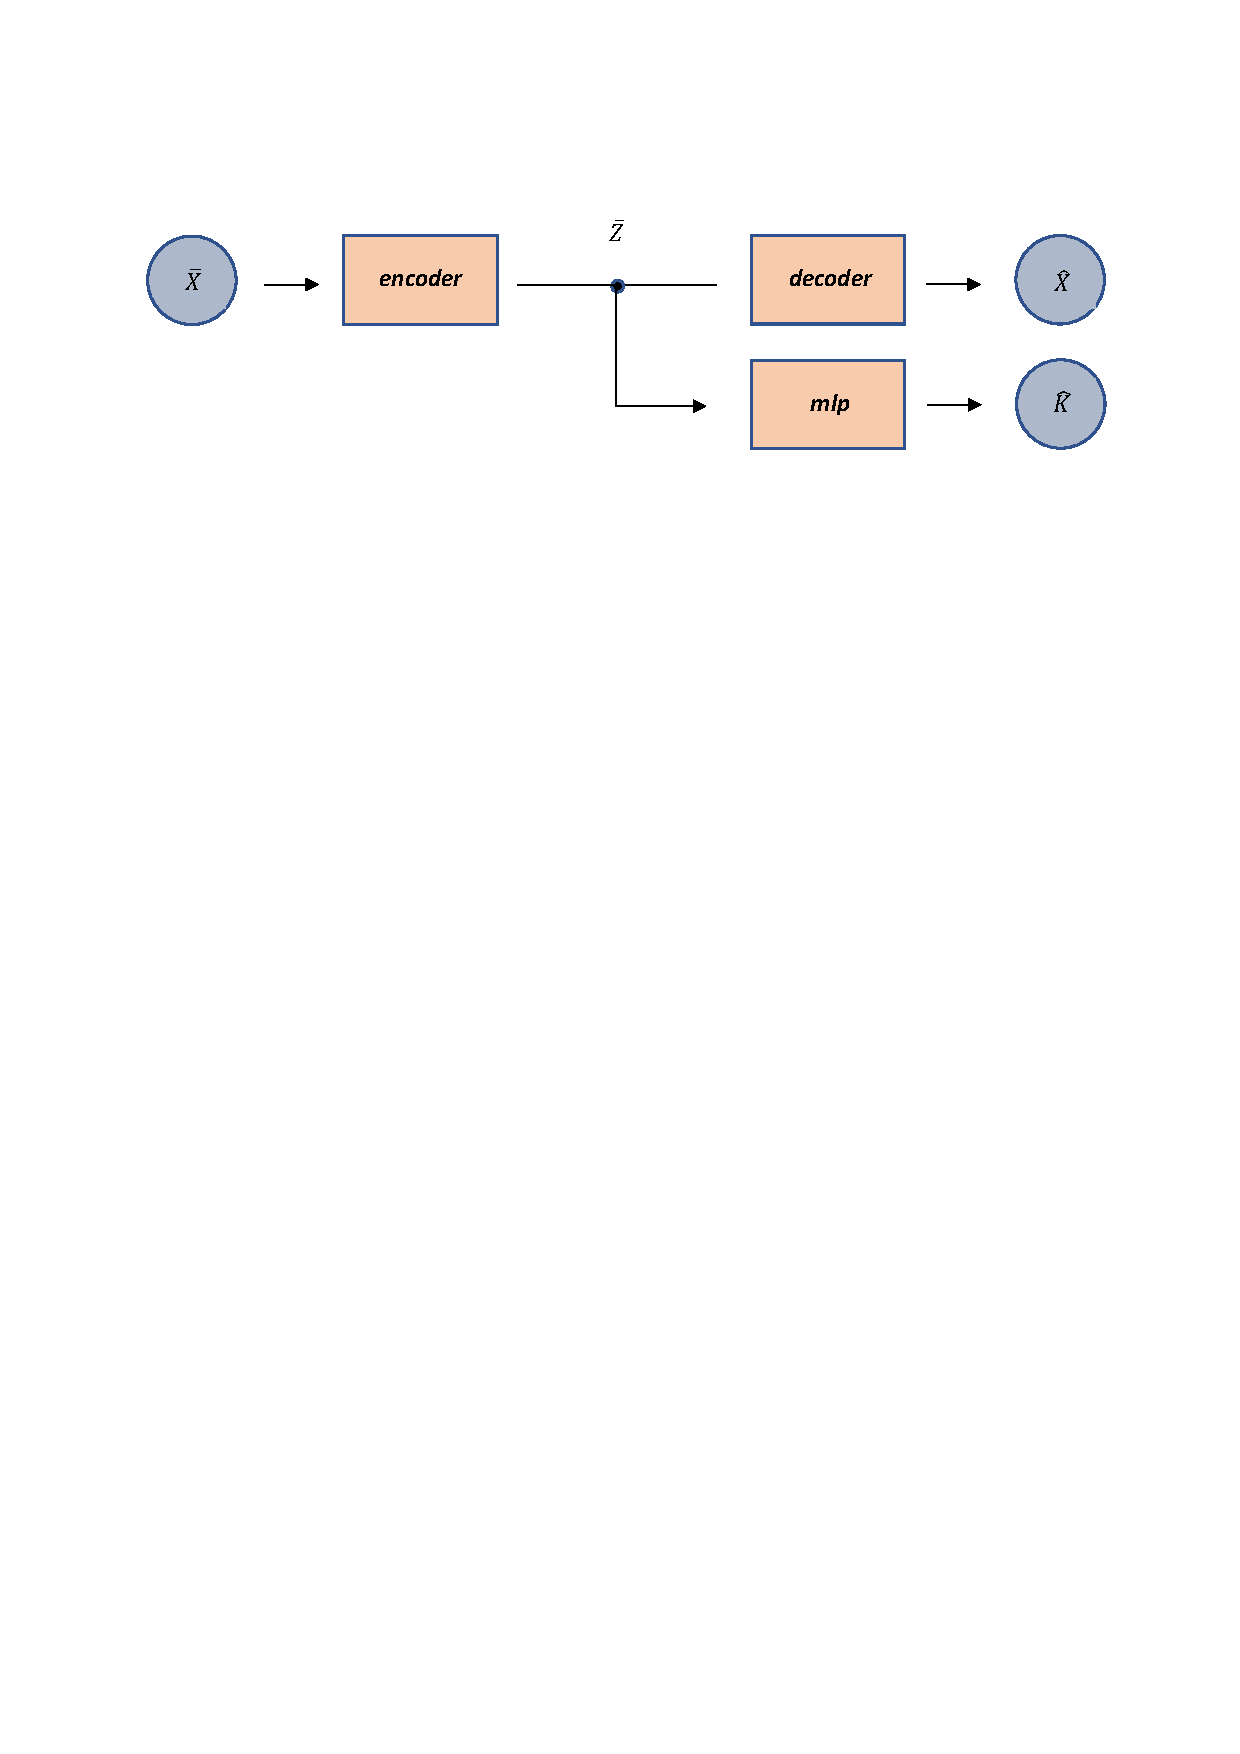
\includegraphics[width=\linewidth]{Figuras_tfg/Diagram_auto_mlp}
  \caption{Autoencoder and MLP.}
  \label{fig:FigA_Autoencoder_MLP} 
\end{subfigure}

\begin{subfigure}{0.98\linewidth} 
  \centering
  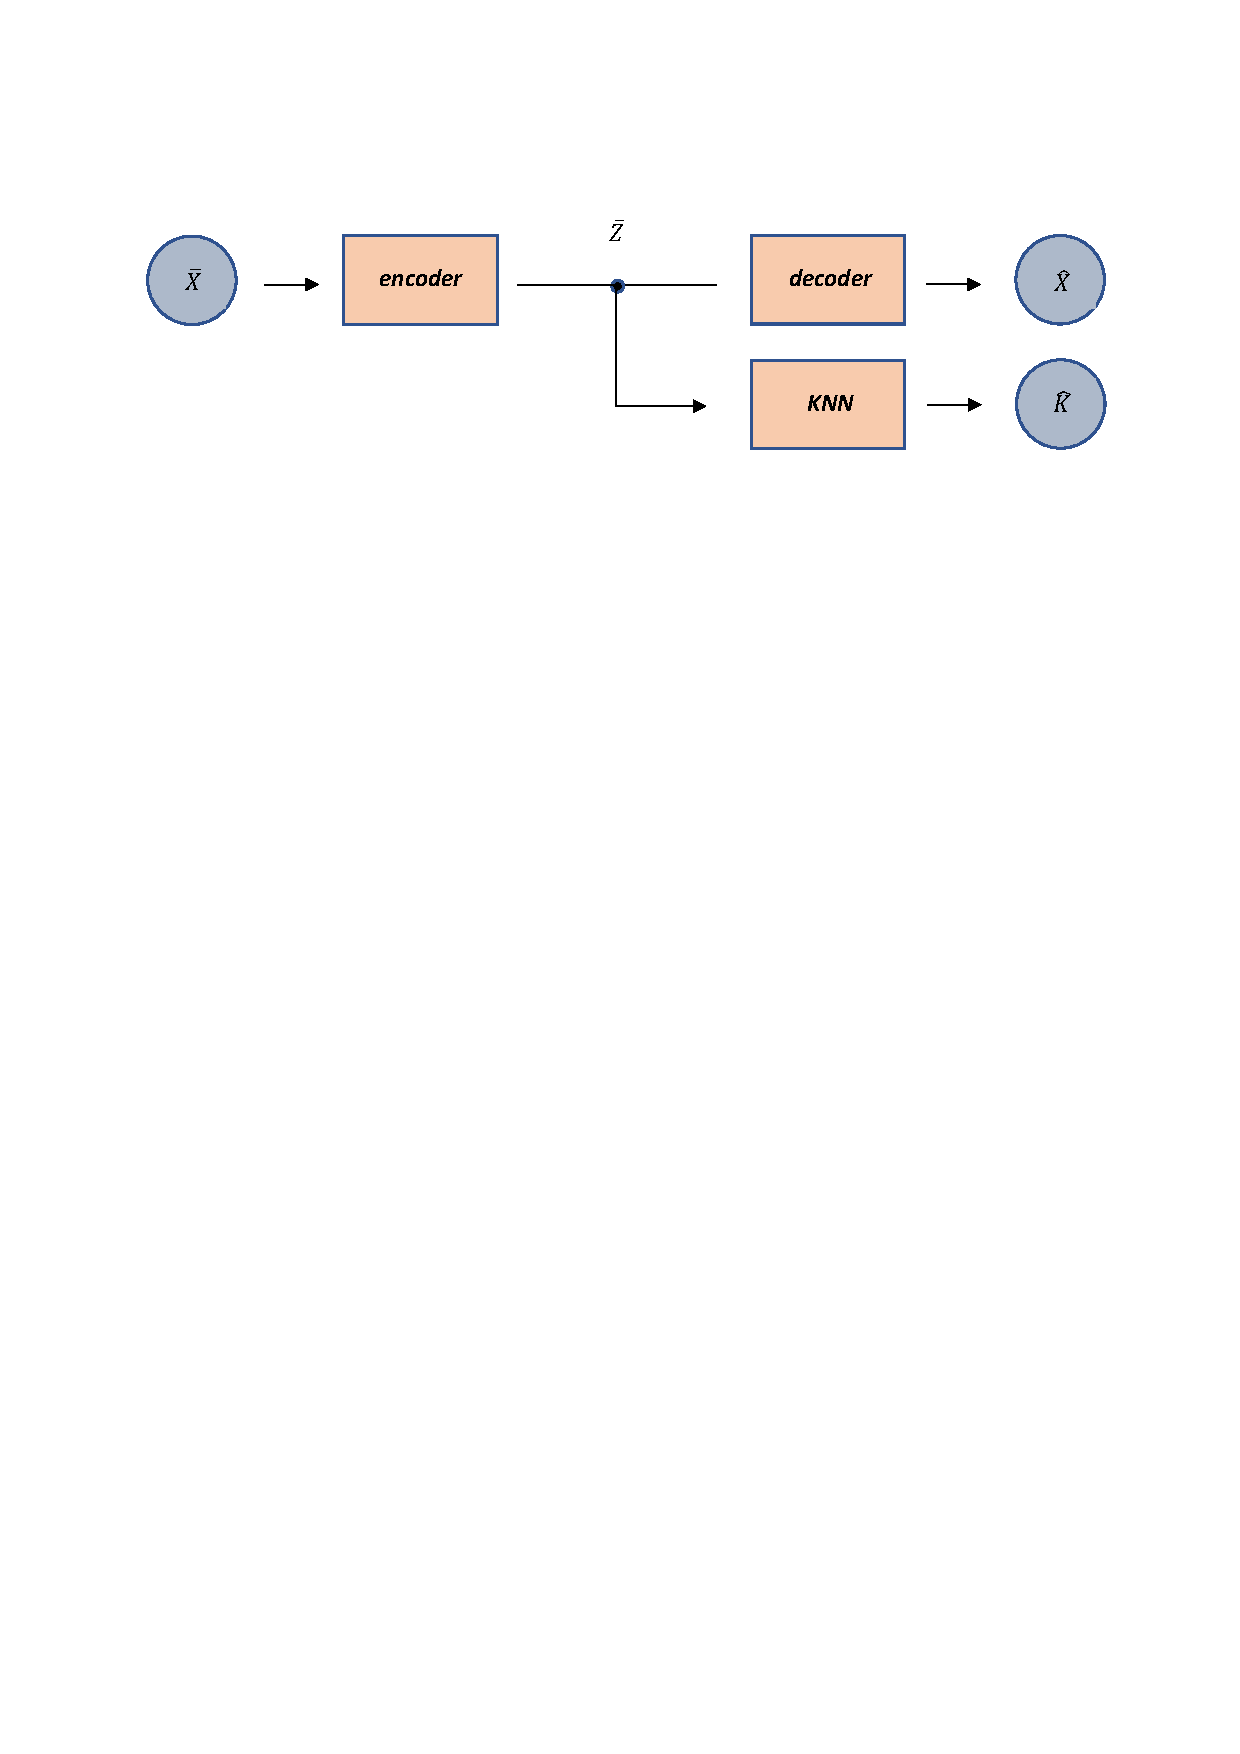
\includegraphics[width=\linewidth]{Figuras_tfg/Diagram_auto_KNN}
  \caption{Autoencoder and KNN.}
  \label{fig:FigB_Autoencoder_KNN} 
\end{subfigure}
  \caption{Structure of the Autoencoder and it's classifiers}
 \label{fig:Autoencoder_architecture}
\end{figure}

We want to compare the effectiveness of the Autoencoder and PCA (see Section~\ref{tools:pca}) to obtain a ``good'' representation for the input. 
%If we compare both diagrams presented here, we 
We can see in Figure~\ref{fig:PCA_architecture} that we use the output from the PCA as the input of the same classifiers as before %, as well as that we will have the same classifiers used in both architectures, 
with the aim to be able to compare their results. 
%
\begin{figure}[H]
\begin{subfigure}{1\linewidth}  
 \centering
  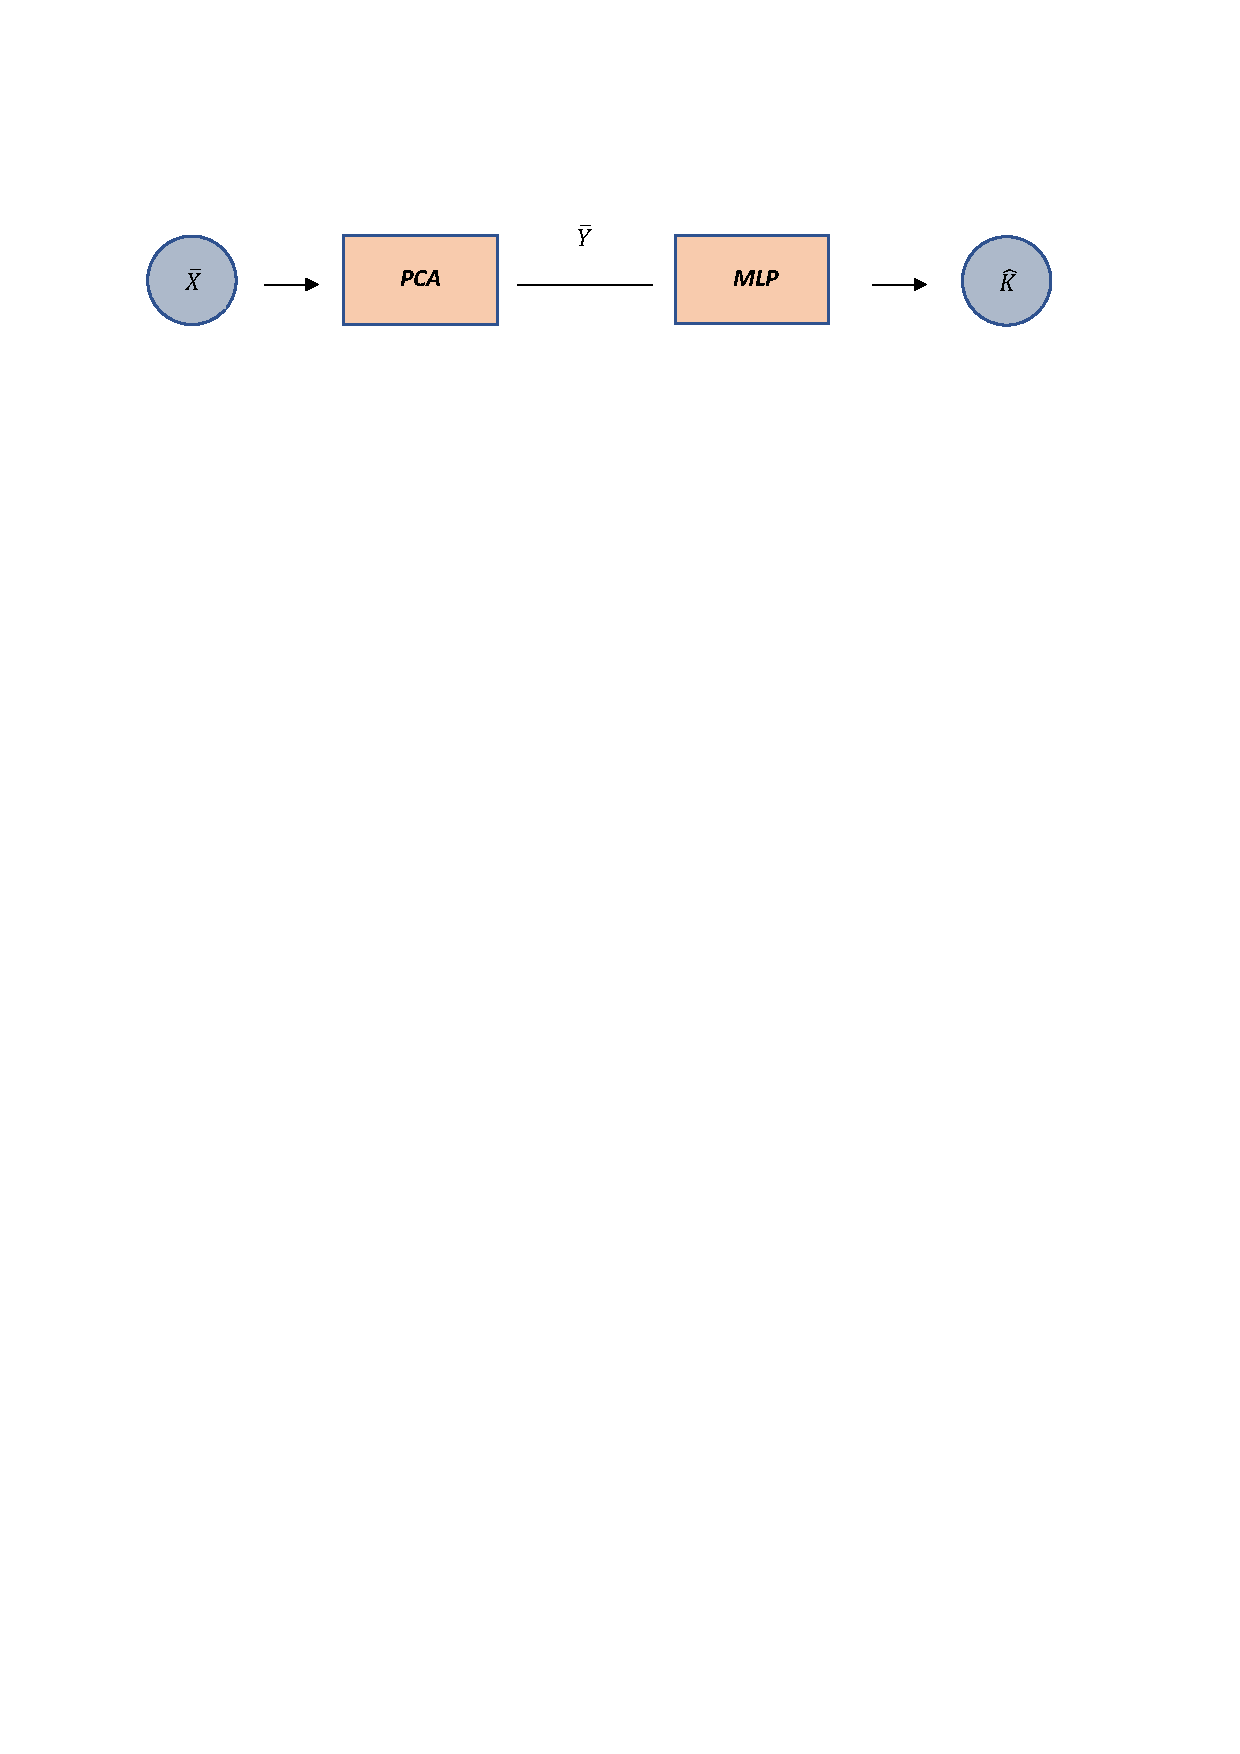
\includegraphics[width=\linewidth]{Figuras_tfg/Diagram_pca_mlp}
  \caption{PCA and MLP.}
  \label{fig:FigA_PCA_MLP} 
\end{subfigure}

\begin{subfigure}{1\linewidth} 
  \centering
  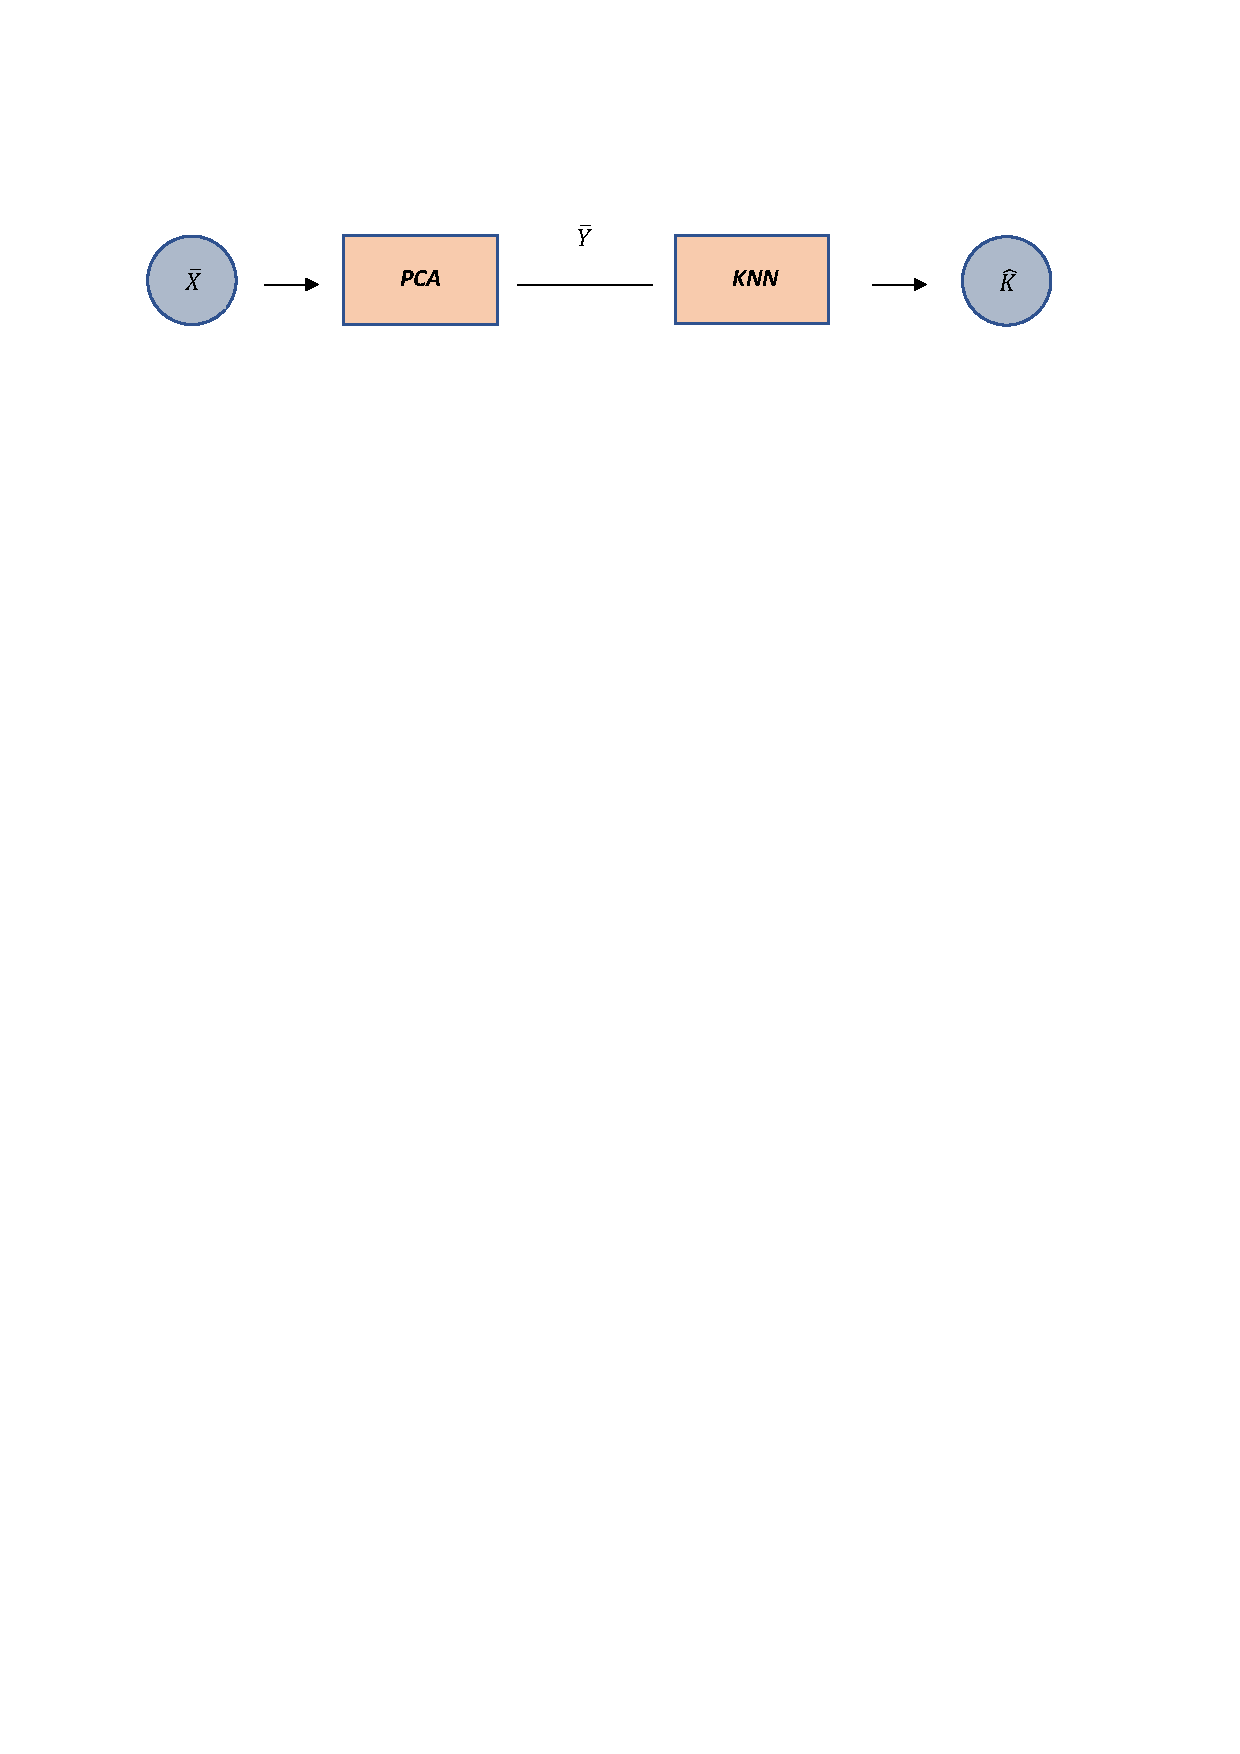
\includegraphics[width=\linewidth]{Figuras_tfg/Diagram_pca_KNN}
  \caption{PCA and KNN.}
  \label{fig:FigB_PCA_KNN} 
\end{subfigure}
  \caption{Structure of the PCA and its classifiers}
 \label{fig:PCA_architecture}
\end{figure}

To increase the reliability of the results we will use 
%As we are also concern about the reliability of them too, we will be including another technique to try to validate our results as much as possible: 
$k$-Fold validation~\cite{mur:12}. 
%
This is a technique
%$k$-Fold is a method which is 
based on dividing a dataset into $k$ disjoint subsets of samples---or ``folds''. We are interested in measuring how each of the architectures performs in each fold of our datasets when training or ``fitting'' the classifiers involved in the other $k-1$ folds. By doing so we obtain---on less training data, that is the $k-1$ folds---an estimate of the performance of the system involved in the retained fold; by repeating this over all of the folds we can also estimate an average and the dispersion of these measures. 
%
Importantly, we can use this technique \emph{on the whole data} at the cost of a slightly increase of the data-dependence of the results.
Using $k=5$ means that we use 5 times $80\%$ of the data for training and $20\%$ of the data for testing. 

% them through the structures presented in both Figure~\ref{fig:Autoencoder_architecture} and~\ref{fig:PCA_architecture}. 
%Once we have each one of them complete the full training process, we will analyse the output plus the summation of the overall results. 

Our hypothesis is that each fold experiment will  provide us with similar data and results in our plots when we use balanced datasets. However, if we have unbalanced datasets we expect to see more inconsistency through them.

The Iris dataset experiment will be thoroughly described and explained as we will be using it as an example of to perform the methods and theory explained on the previous chapters of the report. The remaining experiments will avoid unnecessary explications regarding concepts re-used from the Iris experiment.

At the end of each section, the overall performance of each dataset will be tested with the Entropy Triangle, which will be used to compare the entropy between the data of each Fold and the output of used classifier.

\todo[inline]{So far 20/09/2019}


\section{Iris Dataset}
\subsection{Data Preparation}

In order to train the data through the Autoencoder, we will firstly have to transform it into an easier shape which will reduce the difficulty and length of our task. Normally, Deep Neural Networks will do a good job as long as the data has a reasonable scalability, so applying a normalization to our data is not mandatory. However, it is easier for us to use a simple pre-processing in our data, which given that the observations from the variables have different ranges of values will help us reduce the training time of our Autoencoder.

Although as we can see from Figure \ref{fig:figure_pairs_iris} and Table \ref{tab:table_Iris}, some of its features are closer to what it could be referred as a Normal distribution, specially Sepal Length and Sepal Width. Other variables, such as Petal Length, are a little bit off and far away from that description. To be able to fix those disparities, we will apply a Box-Cox transformation, which consist basically of applying the following equation on your data:

\begin{equation}
\label{eq:box-cox}
 {y(\lambda)=} \left\{
 \begin{aligned}
        \frac{y^{\lambda} - 1}{\lambda} ,  if \  \lambda \neq 0\\
        {\log y}, if \ \lambda = 0
       \end{aligned}
 \right\}
 \end{equation} 
\newline

Where $\lambda$ is an exponent with a value inside the range $[-5,5]$. The Box-Cox method will automatically assign the value of lambda that fits your dataset the most. This value is selected simply by looking for the optimum value by fitting the equation \ref{eq:box-cox} . \par

Once we apply this function, we can start to see the results on our newly created data by checking its pairs function again:

\begin{figure}[H]
	\centering
	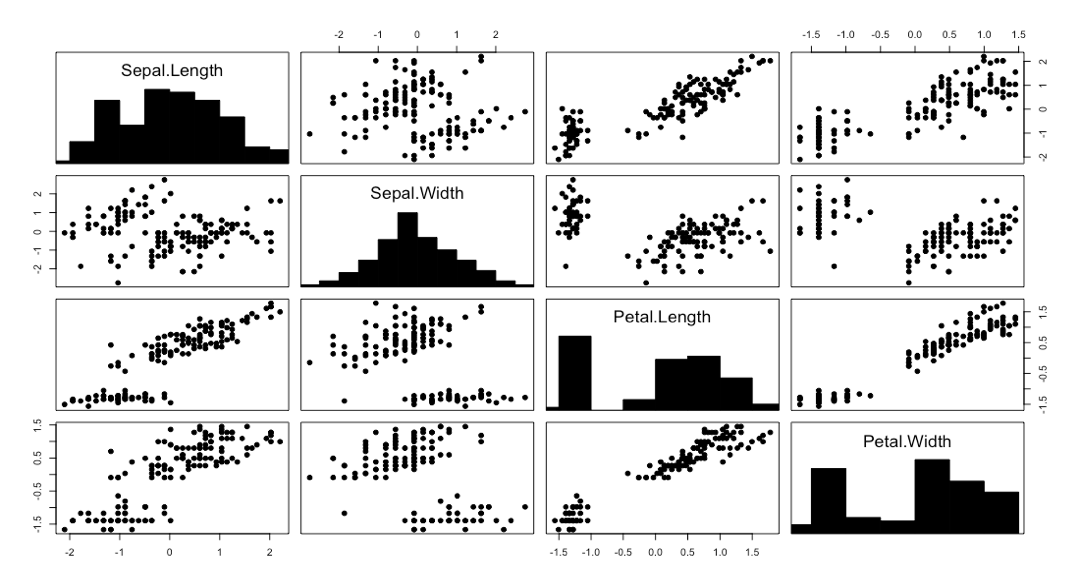
\includegraphics[width=17cm]{Figuras_tfg/Figure_Boxcox}
	\caption{Using the pairs function on Iris Boxcox}
	\label{fig:figure_pairs_iris_bc}
\end{figure}

Which has an histogram slightly different to the one presented on Figure \ref{fig:figure_pairs_iris_bc}, but we can really see the new features of our transformation if we use use the summary function and compare its results with respect to the ones obtained before on Table \ref{tab:table_Iris}
\newline

\begin{table}[H]
		\caption{R summary method on Iris Box Cox.}
	\begin{center}
	\label{tab:table_Iris_Boxcox}
		\begin{tabular}{r|c|c|c|c} % <-- Alignments: 1st column left, 2nd middle and 3rd right, with vertical lines in between
			\textbf{Variable name} & \textbf{Sepal Length} & \textbf{Sepal Width} & \textbf{Petal Length} & \textbf{Petal Width}\\
			\hline
			Minimun & -2.10 & -2.75 & -1.56 & -1.66\\
			Median & 0.02 & -0.08 & 0.33 & 0.27\\
			Mean & 0.00 & 0.00 & 0.00 & 0.00\\
			Maximun & 2.20 & 2.75 & 1.78 & 1.45\\
		\end{tabular}
	\end{center}
\end{table}

By looking at the Table on top, it can be seen that as expected the Mean of our distribution switched from it's previous value to 0, essentially telling us that the transformation has been successful. It is also important to point out that although the values of the vector that are in our dataset are different, we still hold the same proportions and plots of the observations, which means that the general information that each of our variables contained its still there. We just shaped it differently so that it is easier for us to work and perform operations with them.

\subsection{The Autoencoder}

For the Iris dataset, we will use a simple Autoencoder, with just a few layers, that should be enough to complete the training required. As our given dataset doesn't contain a lot of observations, this approach to the Autoencoder aims to show an example of use. That is why, if we take into account that we only have four variables to compress, we can see that the maximum compression we can achieve is a 25 \% of the original size. But, in order to be sure we have a working architecture, I will be using just a 75 \% compression in the middle layer. On the other hand, our model will have a data expansion of about a 400 \%, so that we are able to do a real compression in each of the subsequent layers. \par

\begin{figure}[H]
	\centering
	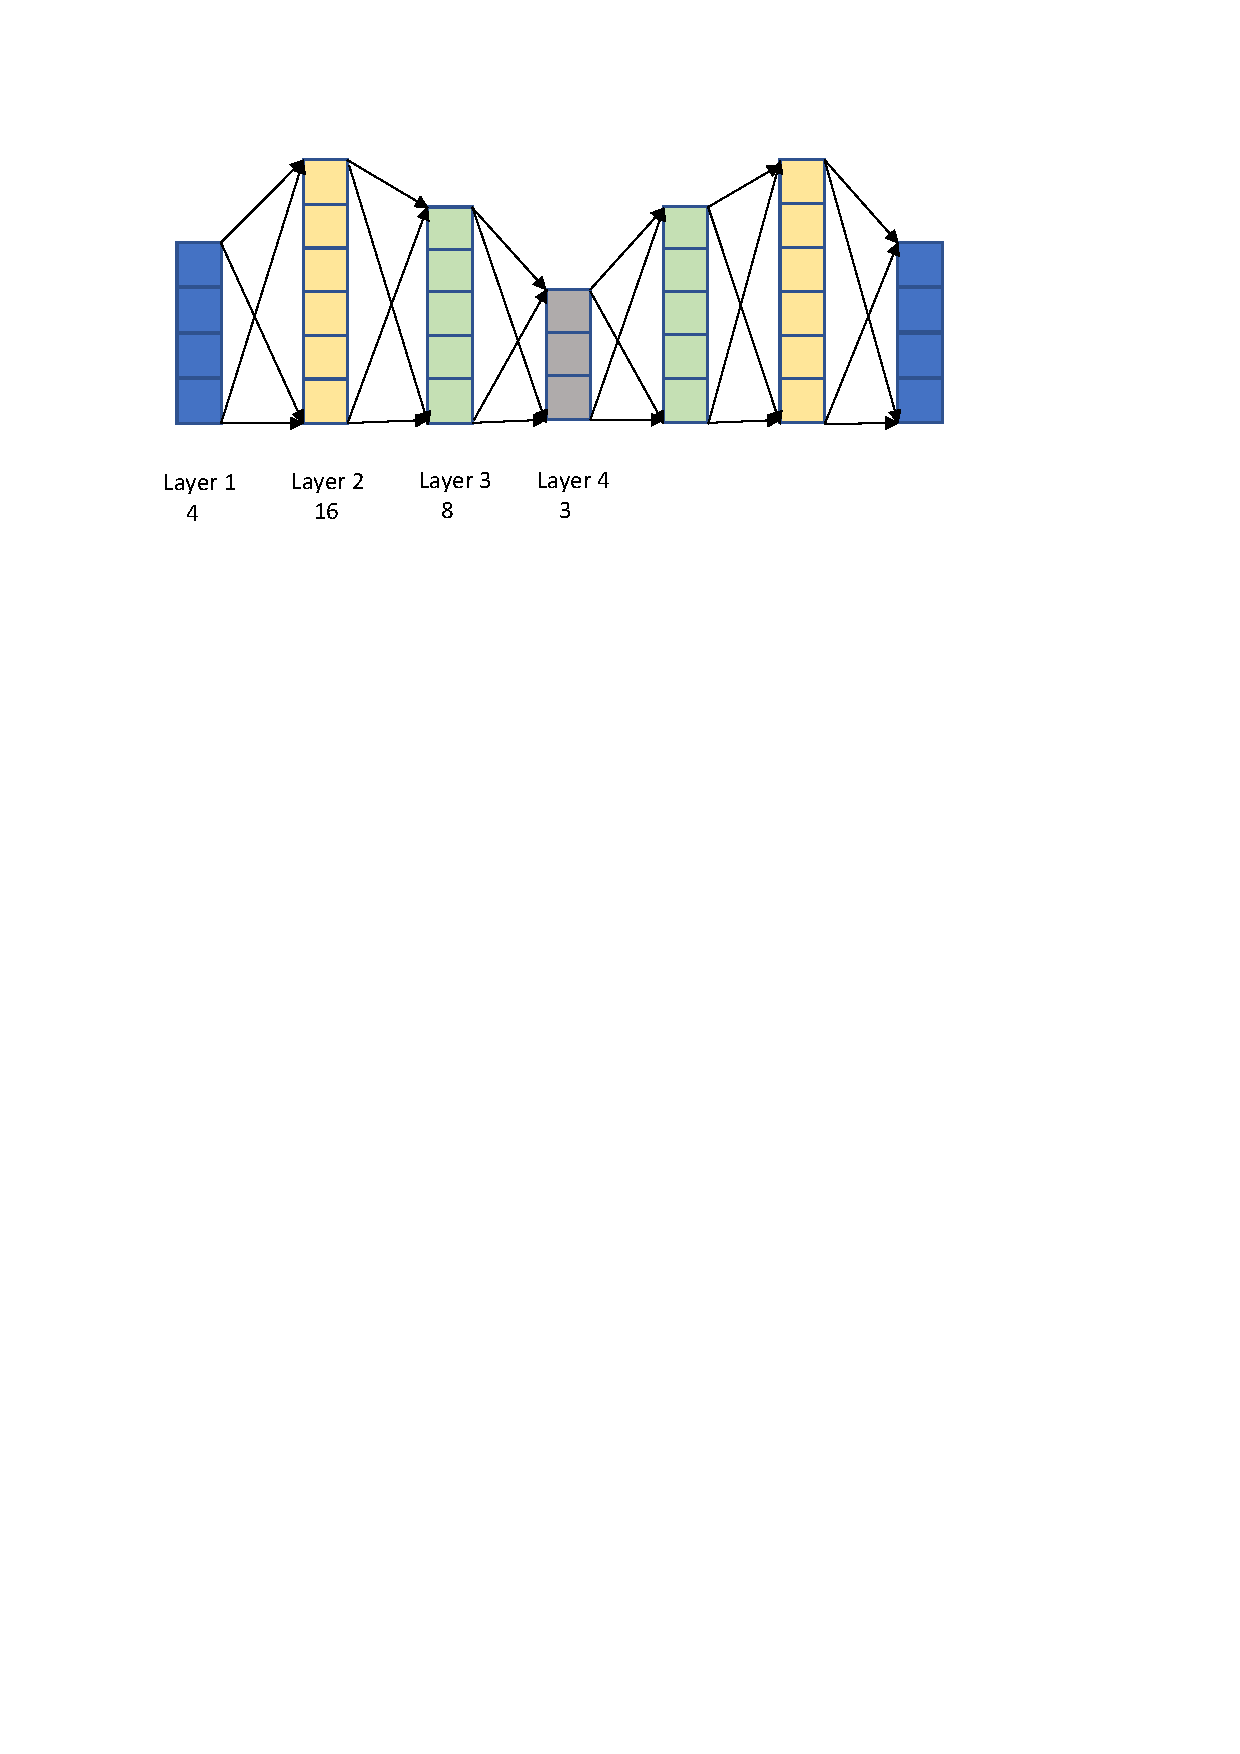
\includegraphics[width=17cm]{Figuras_tfg/Autoencoder_Results}
	\caption{Architecture of the Autoencoder in Iris}
	\label{fig:figure_autoencoder_Iris}
\end{figure}

On Figure \ref{fig:figure_autoencoder_Iris}, each of the layers has the size assigned below it. But before choosing the compilation method we are going to use for the Autoencoder, we have to choose the activation functions for each layer. In this case, we decided that the Relu function would be used \textbf{for all the layers of the Autoencoder except the last one}, where we will use a Sigmoid function. We decided to use this setup because the Relu function does a good job at selecting the informational qualities of each component while at the same time keeping the training time of the architecture very low due to the simplicity of its definition, while the Sigmoid function is more complex and thus seems to be suited for the last layers and to finalize the transferring of information. \par

The last thing to take into account is the compilation of the whole structure created with the previously mentioned Autoencoder. Here, we will have to choose between the wide range of available options on the keras package in R, to try to maximize the performance and optimization of our model. To do so, we have to first rule out all the loss functions that don't apply to our task. For example, although used in a lot of DNNs, the categorical functions don't fit our criteria since we are not performing a classification task here. Moreover, our range of data is not between 0 and 1, which would make this even a worst choice. For us, since we also are trying to predict the output data using some training data, we can assume we have a \textbf{regression problem} in our hands.\par

Having established that, we have a narrower set of possible choices to make. Between all of the left available ones, we decided to use the \textbf{Mean Squared Error function}. The MSE is calculated as the average of the squared differences between the predicted and the original values. This means that the bigger the difference,  more punitive this metric is for our model. This works great for the intent of our experiments, since we want our model to be able to get very accurate predictions from the compressed version of our data. \par

Finally, we also need to decide on our optimizer for the compilation. Here we decided to narrow our options to chose only between the Adam and the Adadelta. Finally, it was seen that the Adam optimizer was achieving the same level of losses as the Adadelta, while needing less epochs. Due to the amount of passes that we have to do through the Autoencoder, it is useful for us to get reliable data in the shortest time possible, so it was finally implemented using Adam.This decision would allow us to help mitigate the problem of time, which can be quite demanding when dealing with multiple transformations and neural networks.

\subsection{The Classifiers}

\subsubsection{Knn on PCA and Autoencoder}
Once we have obtained the output of our Autoencoder, we have a resulting data frame with the same number of observations but a reduced number of variables, which in the case of the Iris Autoencoder will be three, making our resulting matrix to have a shape of $120\times3$. It also must be notest that the process is the same for both the output of the Autoencoder and the PCA.\par

The matrices resulting from this compression process may not have all of their columns or rows with a value different from 0. This does not pose a threat to our training, since none of the methods chosen for our training will drop our results. In the case of the Knn  we will get some Warnings, but as we will see later it won't affect the result of the process. \par


\begin{figure}[H]
	\centering
	\includegraphics[width=15cm]{Figuras_tfg/Knn_example}
	\caption{Knn example on Iris}
	\label{fig:figure_Knn_Iris}
\end{figure}

The function that we decided to use for our Knn training was provided in the train method in the caret package. It only requires you to specify the training data, labeled as x, the labels to be trained with, named as y, and the method, which is a simple Knn classifier. Once provided, the function will start to train your model. \par


Once the model has finished training, we will use the model generated with our values to predict the labels of our model and compare it to the labels used to train it on the first place. Once we have calculated that, we will use the confusion Matrix function to asses the accuracy of our predictions when compared to our original labels. A Confusion Matrix is a table with the same number of columns and rows as your class labels, being the only difference that the diagonal represents the predictions from your model and the class labels that matched, while anything outside of it accounts for the number of missed predictions with respect to the class. In this case, this method will provide us with a $3\times3$ matrix which we then can feed to the jentropies method. \par


\begin{figure}[H]
	\centering
	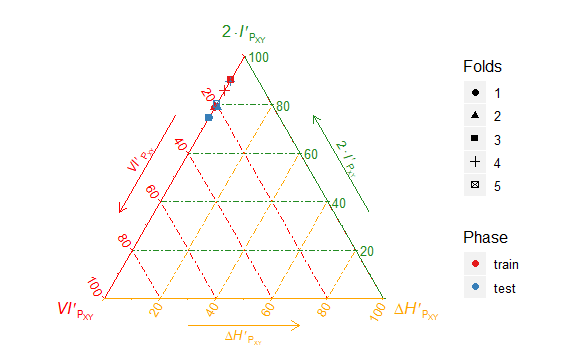
\includegraphics[width=\linewidth]{Figuras_tfg/ET_knn_iris_auto}
	\caption{Entropy Triangle using Autoencoder + Knn in Iris}
	\label{fig:figure_Knn_Iris_ET_Auto}
\end{figure}

\begin{figure}[H]
	\centering
	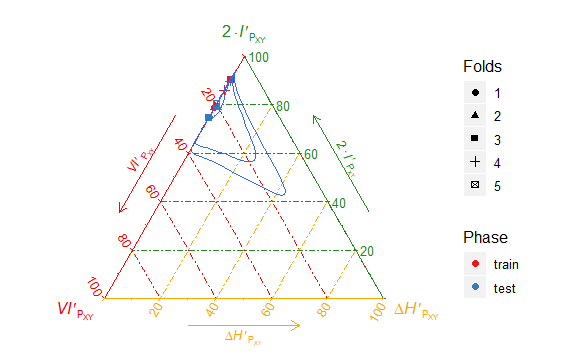
\includegraphics[width=\linewidth]{Figuras_tfg/ET_knn_iris_auto_confidence}
	\caption{Entropy Triangle confidence interval using Autoencoder + Knn in Iris}
	\label{fig:figure_Knn_Iris_ET_Auto_Confidence}
\end{figure}

\begin{figure}[H]
	\centering
	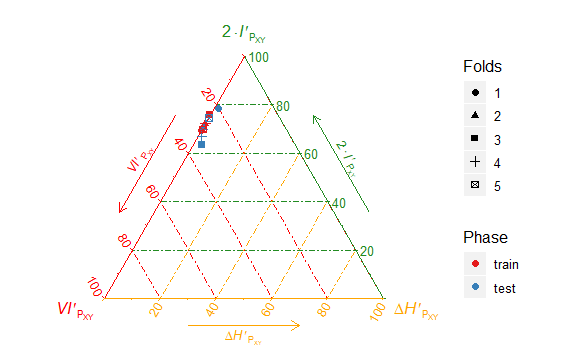
\includegraphics[width=\linewidth]{Figuras_tfg/ET_knn_iris_pca}
	\caption{Entropy Triangle using PCA + Knn in Iris}
	\label{fig:figure_Knn_Iris_ET_PCA}
\end{figure}

\begin{figure}[H]
	\centering
	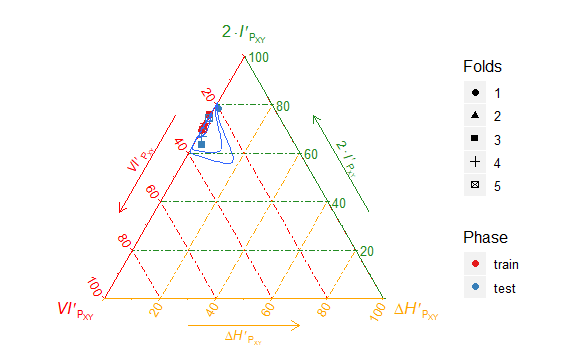
\includegraphics[width=\linewidth]{Figuras_tfg/ET_knn_iris_pca_confidence}
	\caption{Entropy Triangle confidence interval using PCA + Knn in Iris}
	\label{fig:figure_Knn_Iris_ET_PCA_Confidence}
\end{figure}

 Given that we are using a K-Folds validation with a value of $K = 5$, we are plotting 5 coordinates for our test and train variables, just to see how well our model performed.\newline

From Figure \ref{fig:figure_Knn_Iris_ET_Auto} we can see that the values are spatially close inside of the Entropy Triangle. This leads us to believe that the training has been accurate. We usually tend to expect the training and the testing folds to be close if the training process has a balanced set with distinguishable traits differentiating each class from the rest. From the coordinates plotted in the Triangle we can also see that our transformation and classification process has been successful at transmitting the information. By following the guidelines from \ref{chap:BasicPrin} we have a balanced classifier predicting accurately the labels of our classes.  \par

From Figure \ref{fig:figure_Knn_Iris_ET_PCA} we can asses that the conclusions drawn from the Knn of the Autoencoder can also be applied for the PCA. Both figures show a similar behavior, although the Autoencoder has slightly better results as its folds representation is situated closer to the peak of the ET.\par

In addition to plotting the entropic characteristics of the variables, it could be also interesting to take a look at Figure \ref{fig:figure_Knn_Iris_ET_Auto_Confidence} and Figure \ref{fig:figure_Knn_Iris_ET_PCA_Confidence}, which represent the Confidence Intervals of the represented points in the Entropy Triangle. By observing it, we can see that the confidence interval for the Knn in the Autoencoder is spatially greater than the PCA one, leading us to believe that the interval of possible values for the Autoencoder is greater and thus subjected to greater changes in the prediction, probably due to the training uncertainty of the Autoencoder and its effect on the value of $\overline{Z}$. 

%\begin{figure}[H]
%	\centering
%	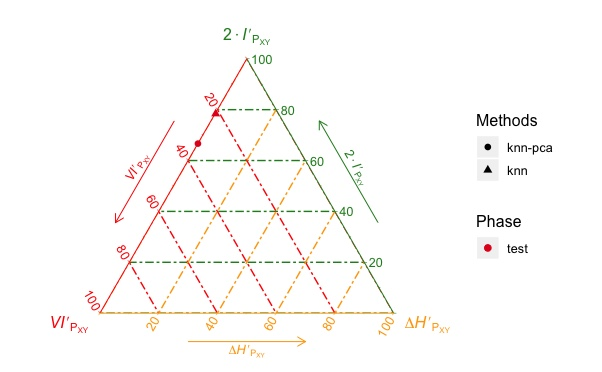
\includegraphics[width=1.2\linewidth]{Figuras_tfg/Total_ET_Knn_Iris}
%	\caption{Entropy Triangle in Knn in Iris with the testing results}
%	\label{fig:figure_Knn_Iris_ET_PCA_Auto}
%\end{figure}

%Although the pca has more consistent and less spread results, we can see in Figure \ref{fig:figure_Knn_Iris_ET_PCA_Auto} that the Autoencoder has done an overall better job at providing information for the knn for the classification. Both of them are placed on the side of Triangle $VI_{P_{XY}}$ that accounts for the transference of information, but the Autoencoder is providing a better representation of the data that is allowing the knn to do a better job overall. \par

%We can therefore conclude that, in the case of the classification using the  knn on both the PCA and the Autoencoder, we have found the latter to do a better job than the first one informationally speaking, thus leaving us with the assumption that it is the preferred solution for the Iris dataset.

\subsubsection{	MLP on PCA and Autoencoder}

Before fitting the data through a MLP, we have to specify the structure that we are implementing on our Neural Network. Seeing that the PCA and the Autoencoder both predict different lengths for our target training matrices, we have to take into account that the input shape will differ. \par

Once we know that, we can start looking at our structure. Since we are dealing again with a small number of variables, a simple approach will be to divide our MLP into 4 layers. Firstly, we place an input layer with the size of our data, either a $3\times120$ in the Autoencoder or a $4\times120$ in the PCA. Secondly, we can place an expansion layer of size 5, followed by the first compression layer of 4, which is connected to the last one which will be the output of our architecture. \par

\begin{figure}[H]
	
	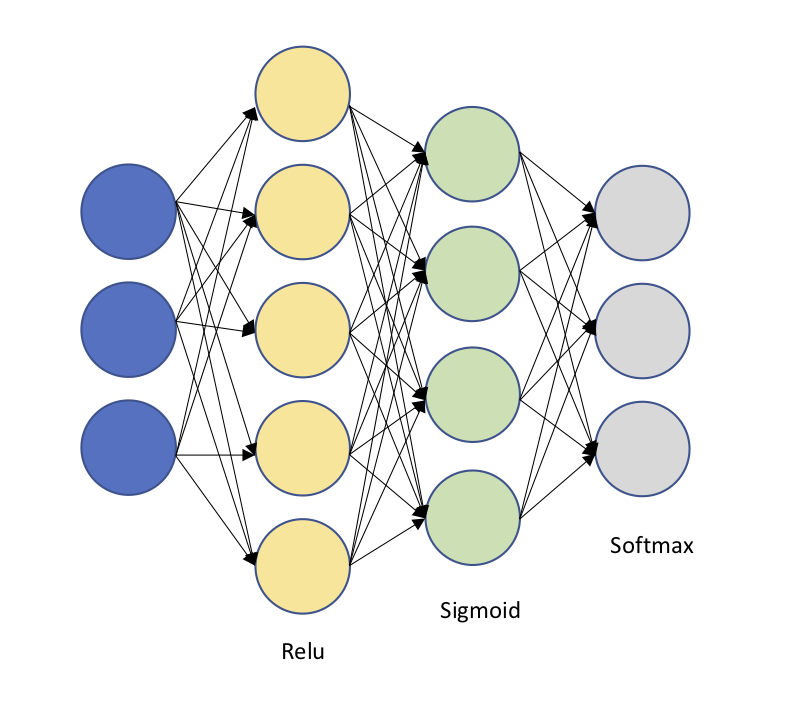
\includegraphics[width=0.8\linewidth]{Figuras_tfg/Example_MLP_Auto.png}
	\caption{MLP architecture in Iris for the Autoencoder}
	\label{fig:figure_MLP_Iris_Autoencoder}
\end{figure}

After figuring out the structure, we now have to decide which activation function would fit the best for each layer. As in the Autoencoder, the first layer will be a Relu, the second one acquires the role of the Sigmoid and finally, as the MLP is a classifier, we have to place a softmax activation function at the end. We want the output of our Autoencoder to be a decision and the softmax is the chosen solution, as we will get our output variables to have an added value equal to 1, being the greater one the label predicted. \par

\begin{figure}[H]
	
	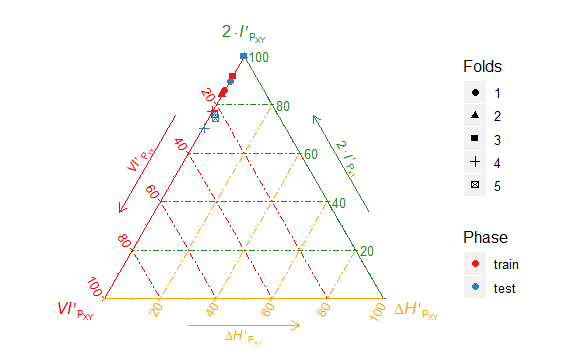
\includegraphics[width=\linewidth]{Figuras_tfg/ET_Iris_Auto_Mlp}
	\caption{Entropy Triangle using Autoencoder + MLP in Iris}
	\label{fig:figure_MLP_Iris_ET_Auto}
\end{figure}

\begin{figure}[H]
	
	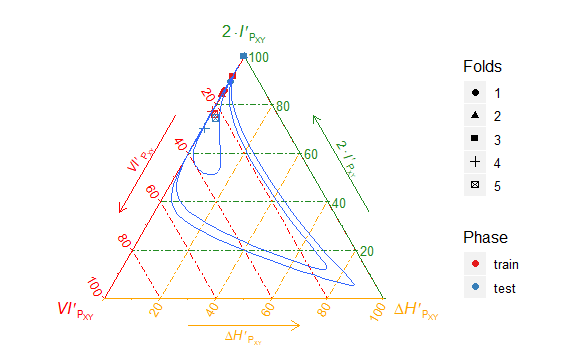
\includegraphics[width=\linewidth]{Figuras_tfg/ET_Iris_Auto_Mlp_Confidence}
	\caption{Entropy Triangle confidence interval using Autoencoder + MLP in Iris}
	\label{fig:figure_MLP_Iris_ET_Auto_Confidence}
\end{figure}

\begin{figure}[H]
	
	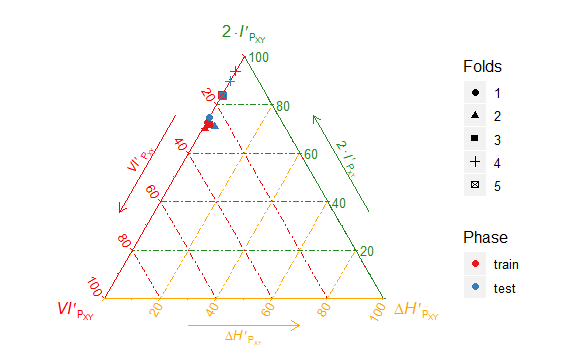
\includegraphics[width=\linewidth]{Figuras_tfg/ET_Iris_Pca_Mlp}
	\caption{Entropy Triangle using PCA + MLP in Iris}
	\label{fig:figure_MLP_Iris_ET_PCA}
\end{figure}

\begin{figure}[H]
	
	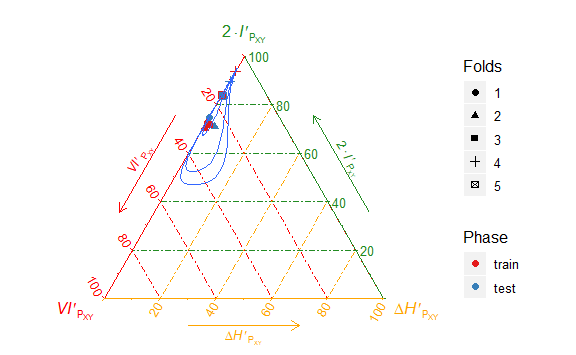
\includegraphics[width=\linewidth]{Figuras_tfg/ET_Iris_Pca_Mlp_Confidence}
	\caption{Entropy Triangle confidence interval using PCA + MLP in Iris}
	\label{fig:figure_MLP_Iris_ET_PCA_Confidence}
\end{figure}

From Figure \ref{fig:figure_MLP_Iris_ET_Auto} we can see that we have obtained more spatially separated points in our ET with respect to Figure \ref{fig:figure_Knn_Iris_ET_Auto} from the previous section. Nevertheless, it seems that the results from the MLP classifier overall show a better performance at classifying our observations than the Knn for the same $\overline{Z}$. We even see that the third testing fold was classified perfectly.

We observe the same spatial separation and behavior on the PCA transformation by comparing again Figure \ref{fig:figure_MLP_Iris_ET_PCA} with \ref{fig:figure_Knn_Iris_ET_PCA}. Again we are obtaining better results than those from the Knn. \par

On the other hand, Figure \ref{fig:figure_MLP_Iris_ET_PCA_Confidence} and Figure \ref{fig:figure_MLP_Iris_ET_Auto_Confidence} have greater confidence intervals than those presented in the previous section. The uncertainty introduced in the predictive process affects this time both the PCA and the Autoencoder, although we see that the training of the Autoencoder added to the training of the MLP has made our confidence interval in Figure \ref{fig:figure_MLP_Iris_ET_Auto_Confidence} increase greatly. Basically, we can see here that without proper training our folds could specialize in predicting certain class rather than being balanced.
 
\subsection{Results discussion} 

After analyzing the Knn and MLP by on its own, we now are going to plot the summation from all of the testing folds in order to get an overall idea about how well each one of our transformations + classifications performed.\par                 

We are using the testing fold only in order to see how well our transformations performed in our data we have to compare the accuracy of its predictions over the whole dataset. We don't need to asses the training as we have already seen on the previous sections that our training folds results in the ET have been consistent with its testing observations. \par

\begin{figure}[H]
	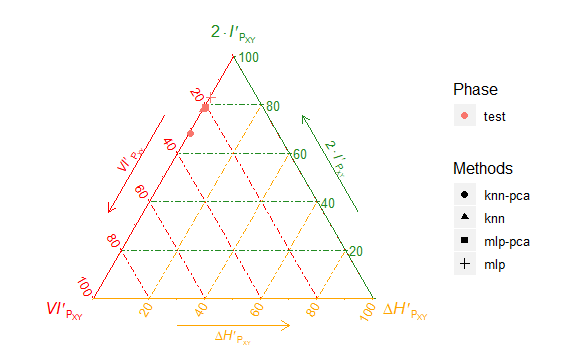
\includegraphics[width=1\linewidth]{Figuras_tfg/ET_Iris_Total_Results}
	\caption{Entropy Triangle in Iris with the total testing result}
	\label{fig:figure_ET_Total_Testing_Iris}
\end{figure}

By looking at Figure \ref{fig:figure_ET_Total_Testing_Iris} the MLP classifier on the Autoencoder seems to have outperformed the rest of the testing structures. The worst one is the Knn in PCA, which is placed lower in the ET. If we consider the reliability of all the classifiers included, we can see that overall all of them do a good job at classifying the Iris datasset. However, the accuracy of the MLP with the Autoencoder outperforms the rest of them.

\section{Ionosphere Dataset}
\subsection{Data Preparation}

The only pre-proccessing done for Ionosphere was explained in Subsection \ref{subsec:Ionosphere} referred to the datasets. No Box-Cox or other method was found to improve the performance on this particular case. We will only get rid of the column with no variance, which as mentioned before was a column with a constant value of 0 all throughout the set. As explained before, we expect this dataset to show more unbalancing in its results.

\subsection{The Autoencoder}

Ionosphere has more variables that Iris, but it is still a small Autoencoder compared to the structure that we are using for MNIST. Our architecture transforms the data provided by the package into 8 observations. We again are using an Autoencoder with the same amount layers structured as:  \newline

\begin{table}[H]
	\caption{Ionosphere Autoencoder layers of the encoder.}
	\begin{center}
		\label{tab:table_Ionosphere_auto_encoder}
		\begin{tabular}{c|c|c} % <-- Alignments: 1st column left, 2nd middle and 3rd right, with vertical lines in between
			\textbf{Number of Layers} & \textbf{Size} & \textbf{Activation Function} \\
			\hline
			First & 33 & None\\
			Second & 50 & Relu\\
			Third & 20 & Relu\\
			Fourth or Middle & 8 & Relu\\
		\end{tabular}
	\end{center}
\end{table}

\begin{table}[H]
	\caption{Ionosphere Autoencoder layers of the decoder.}
	\begin{center}
		\label{tab:table_Ionosphere_auto_decoder}
		\begin{tabular}{c|c|c} % <-- Alignments: 1st column left, 2nd middle and 3rd right, with vertical lines in between
			\textbf{Number of Layers} & \textbf{Size} & \textbf{Activation Function} \\
			\hline
			Middle or First & 8 & Relu\\
			Second & 20 & Relu\\
			Third & 50 & Relu\\
			Fourth or Output & 33 & Sigmoid\\
		\end{tabular}
	\end{center}
\end{table}

As seen of both Table \ref{tab:table_Ionosphere_auto_encoder} and Table \ref{tab:table_Ionosphere_auto_decoder}, with the aim to compare the results provided by both datasets, we are going to use the same compilation options and activation functions as in Iris. We think it would be interesting to test the same compilation environment for two datasets with completely different characteristics.\par

It is expected for Ionosphere to not be difficult to train, since it is very unbalanced and classifiers tend to just choose the predominant class in the dataset as their predicted value in most of the cases. Both the MLP and the KNN suffer from this unwanted tendency, but we want to reproduce that behavior on this experiment.

\subsection{Knn on PCA and Autoencoder}

We will follow the same process to present the results regarded from the Ionosphere dataset:

\begin{figure}[H]
	\centering
	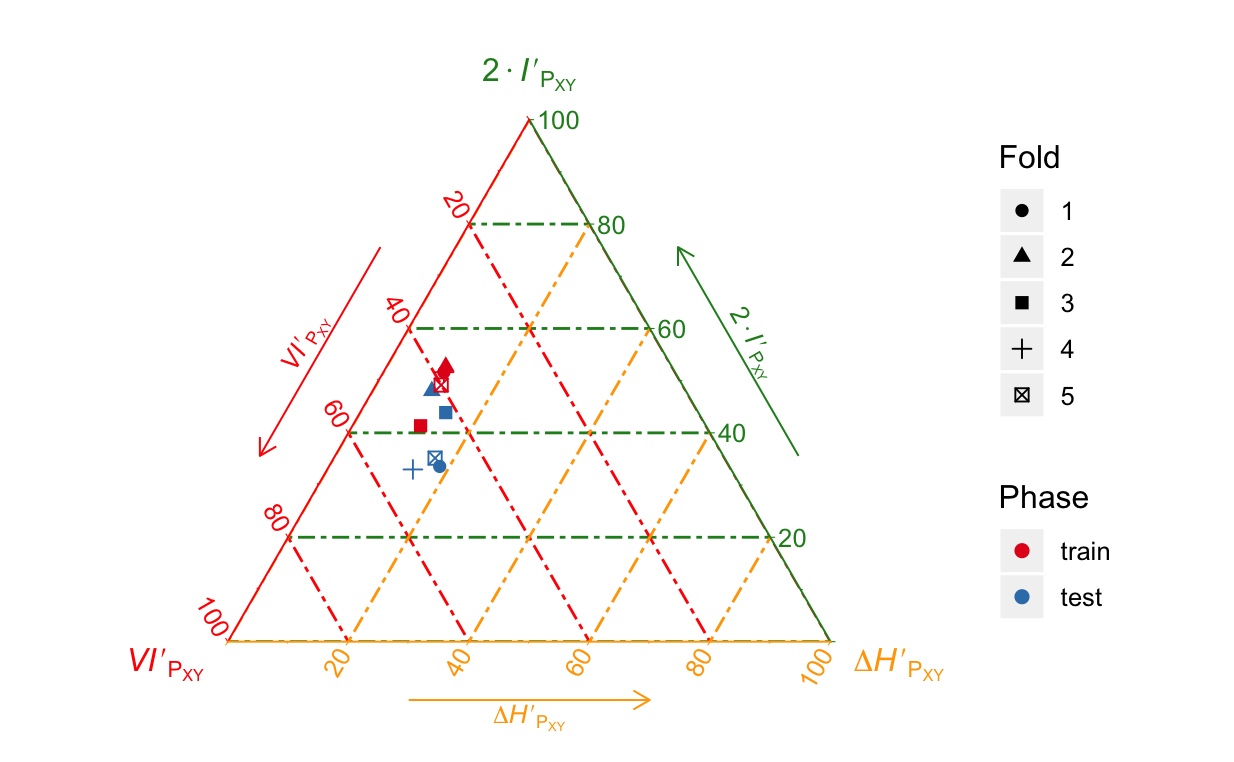
\includegraphics[width=\linewidth]{Figuras_tfg/ET_Iono_Auto_Knn}
	\caption{Entropy Triangle using Autoencoder + Knn in Ionosphere}
	\label{fig:figure_Knn_Iono_ET_Auto}
\end{figure}

\begin{figure}[H]
	\centering
	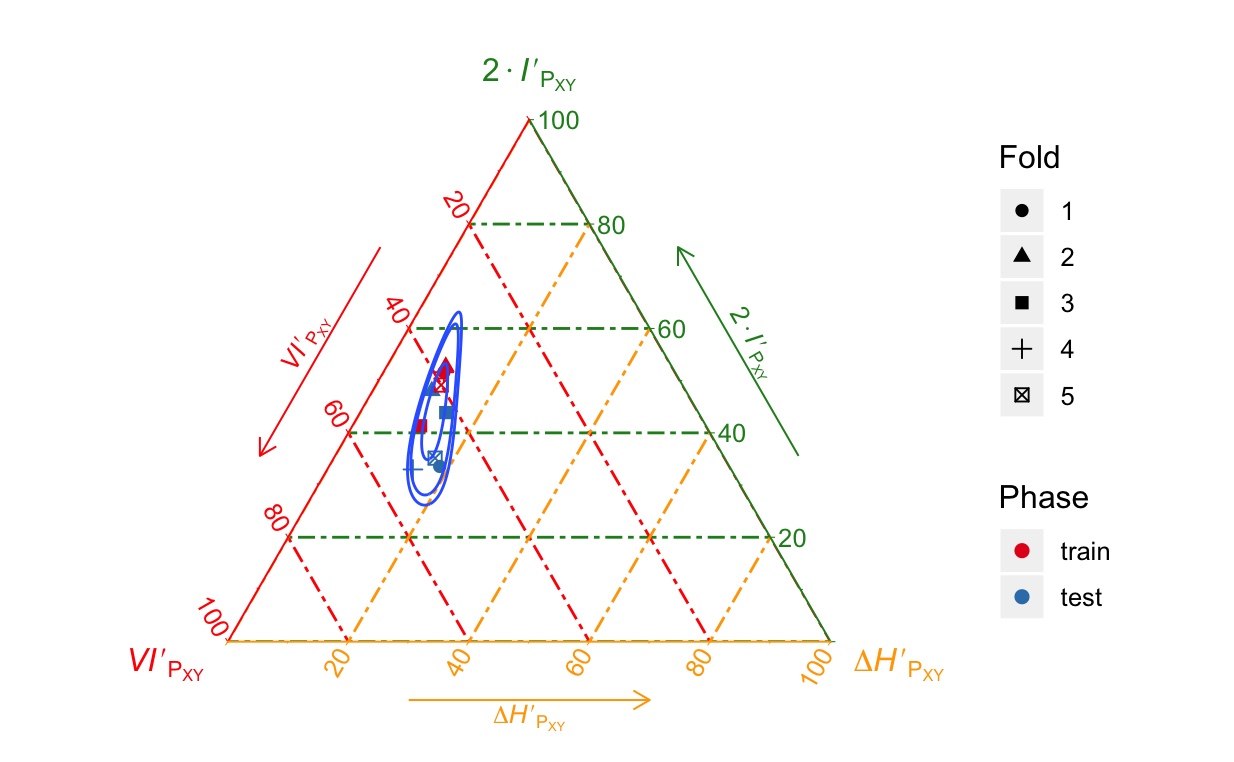
\includegraphics[width=\linewidth]{Figuras_tfg/ET_Iono_Auto_Knn_Confidence}
	\caption{Entropy Triangle confidence interval using Autoencoder + Knn in Ionosphere}
	\label{fig:figure_Knn_Iono_ET_Auto_Confidence}
\end{figure}

\begin{figure}[H]
	\centering
	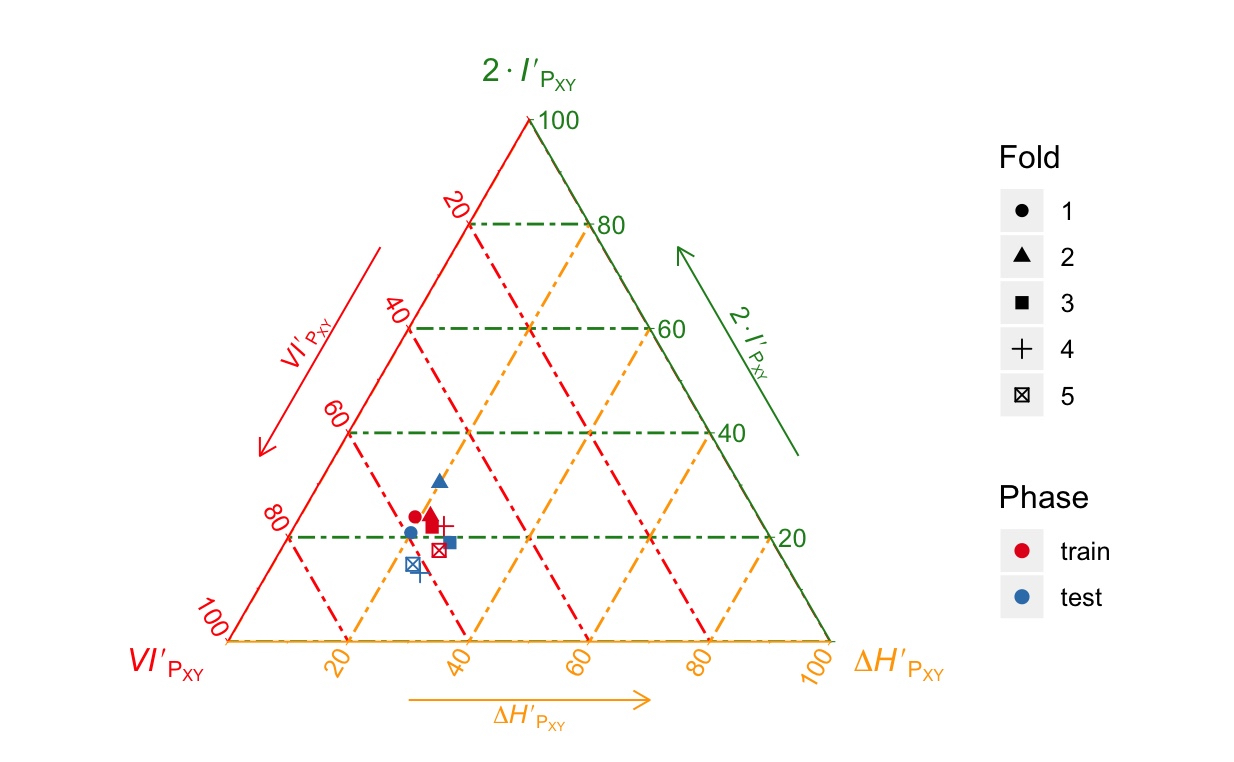
\includegraphics[width=\linewidth]{Figuras_tfg/ET_Iono_PCA_Knn}
	\caption{Entropy Triangle using PCA + Knn in Ionosphere}
	\label{fig:figure_Knn_Iono_ET_PCA}
\end{figure}

\begin{figure}[H]
	\centering
	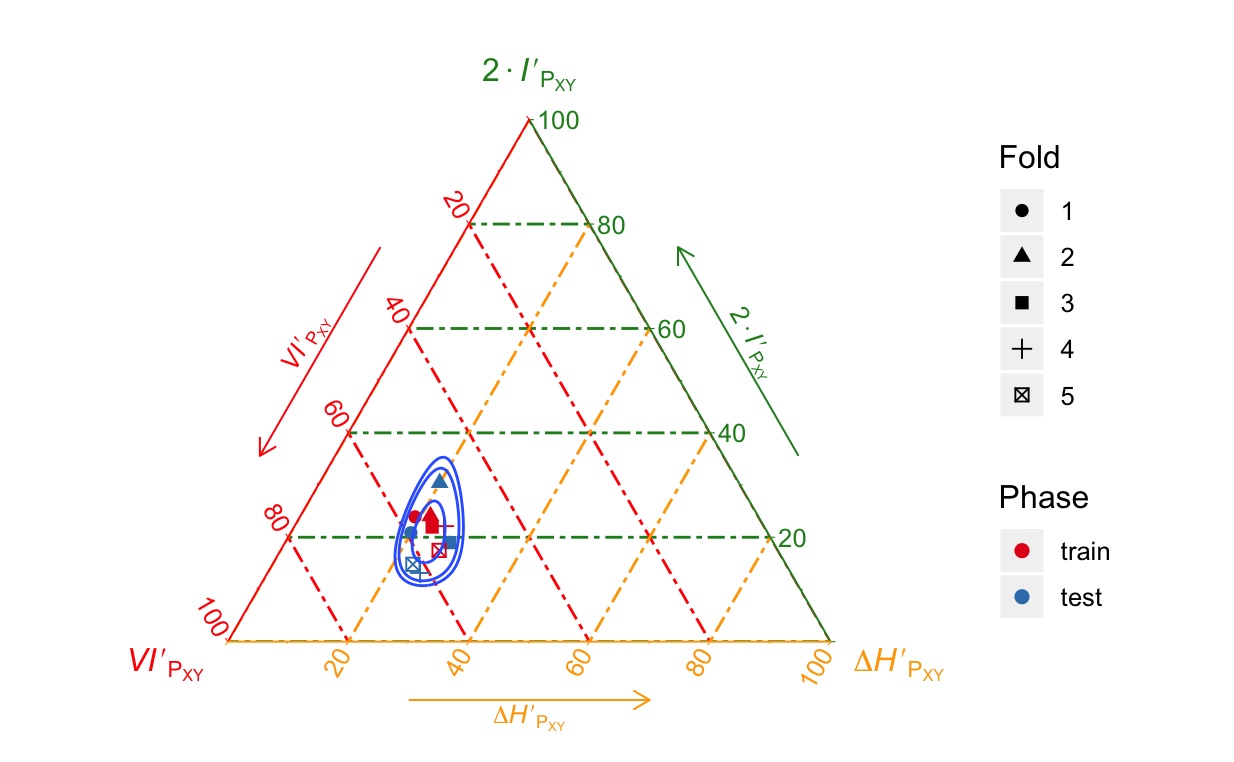
\includegraphics[width=\linewidth]{Figuras_tfg/ET_Iono_PCA_Knn_Confidence}
	\caption{Entropy Triangle confidence interval using PCA + Knn in Ionosphere}
	\label{fig:figure_Knn_Iono_ET_PCA_Confidence}
\end{figure}

Just by taking a simple look over Figure \ref{fig:figure_Knn_Iono_ET_Auto} and Figure \ref{fig:figure_Knn_Iono_ET_PCA} it is noticeable that the unbalancing of the dataset has affected the outcome of our experiments. The coordinates of the entropies from our Knn Folds tells us that our predictions have been inaccurate and the transmission of information either by means of the Virtual Information or the Mutual Information have degraded a lot from the results gathered from the Iris dataset. \par

On the other hand, Figure \ref{fig:figure_Knn_Iono_ET_Auto_Confidence} and Figure \ref{fig:figure_Knn_Iono_ET_PCA_Confidence} point to us that sparsity of possible new test values is not very big, which basically is indicating that our classifications can't greatly vary their inaccurate predictions.\par 

\subsection{MLP on PCA and Autoencoder}

To completely asses the Ionosphere dataset classification process we must now asses the performance of the MLP:

\begin{figure}[H]
	\centering
	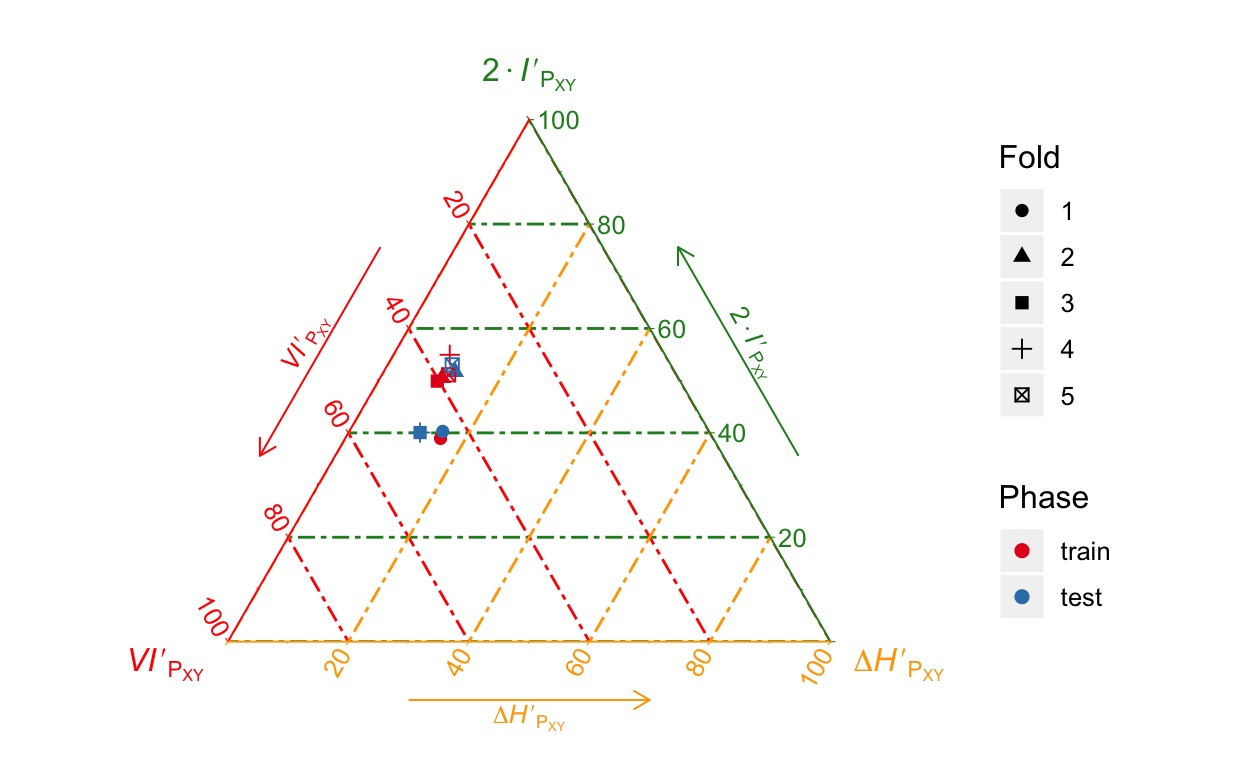
\includegraphics[width=\linewidth]{Figuras_tfg/ET_Iono_Auto_Mlp}
	\caption{Entropy Triangle using Autoencoder + MLP in Ionosphere}
	\label{fig:figure_Mlp_Iono_ET_Auto}
\end{figure}

\begin{figure}[H]
	\centering
	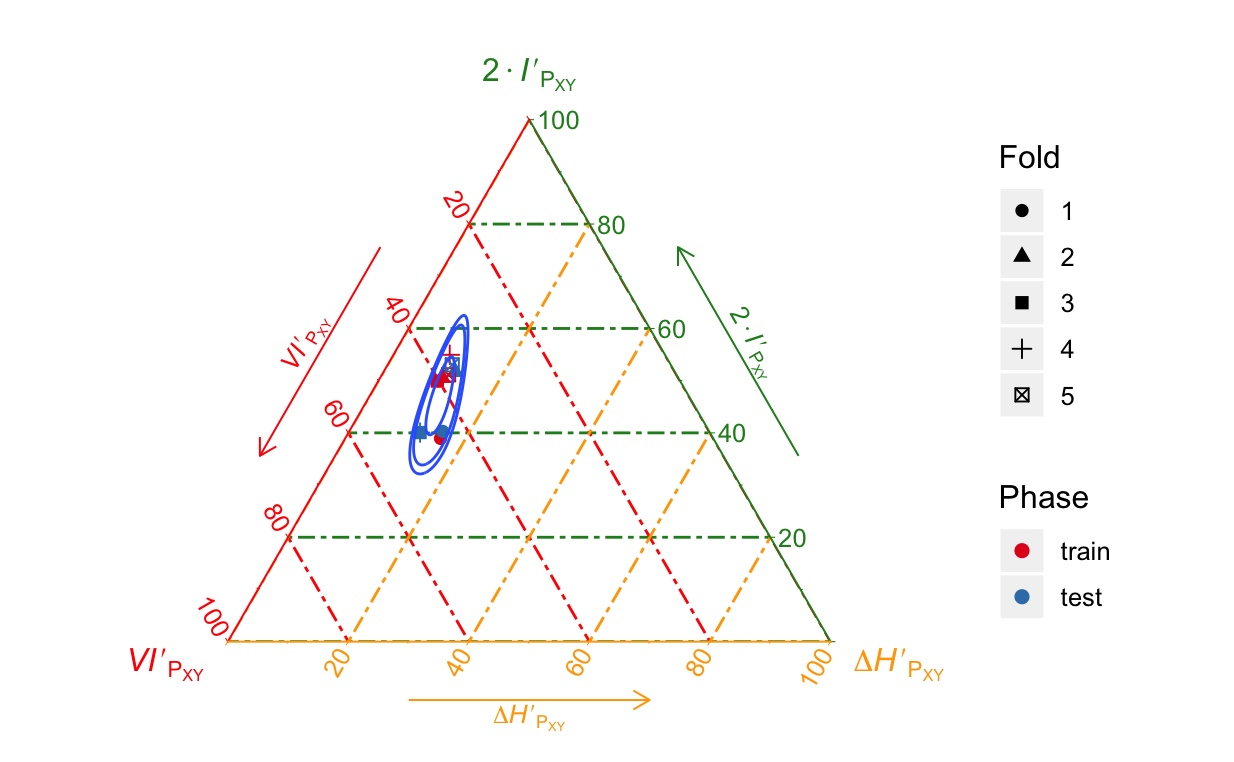
\includegraphics[width=\linewidth]{Figuras_tfg/ET_Iono_Auto_Mlp_Confidence}
	\caption{Entropy Triangle confidence interval using Autoencoder + MLP in Ionosphere}
	\label{fig:figure_Mlp_Iono_ET_Auto_Confidence}
\end{figure}

\begin{figure}[H]
	\centering
	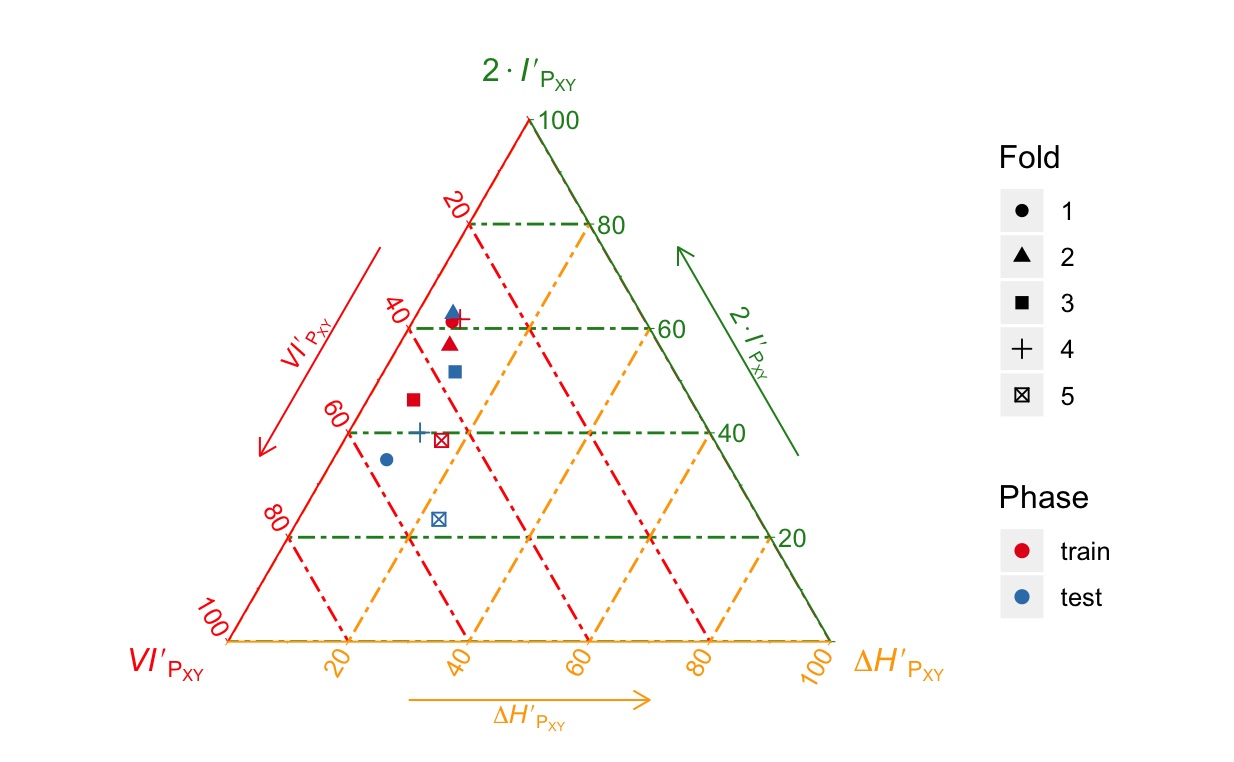
\includegraphics[width=\linewidth]{Figuras_tfg/ET_Iono_PCA_Mlp}
	\caption{Entropy Triangle using PCA + Mlp in Ionosphere}
	\label{fig:figure_Mlp_Iono_ET_PCA}
\end{figure}

\begin{figure}[H]
	\centering
	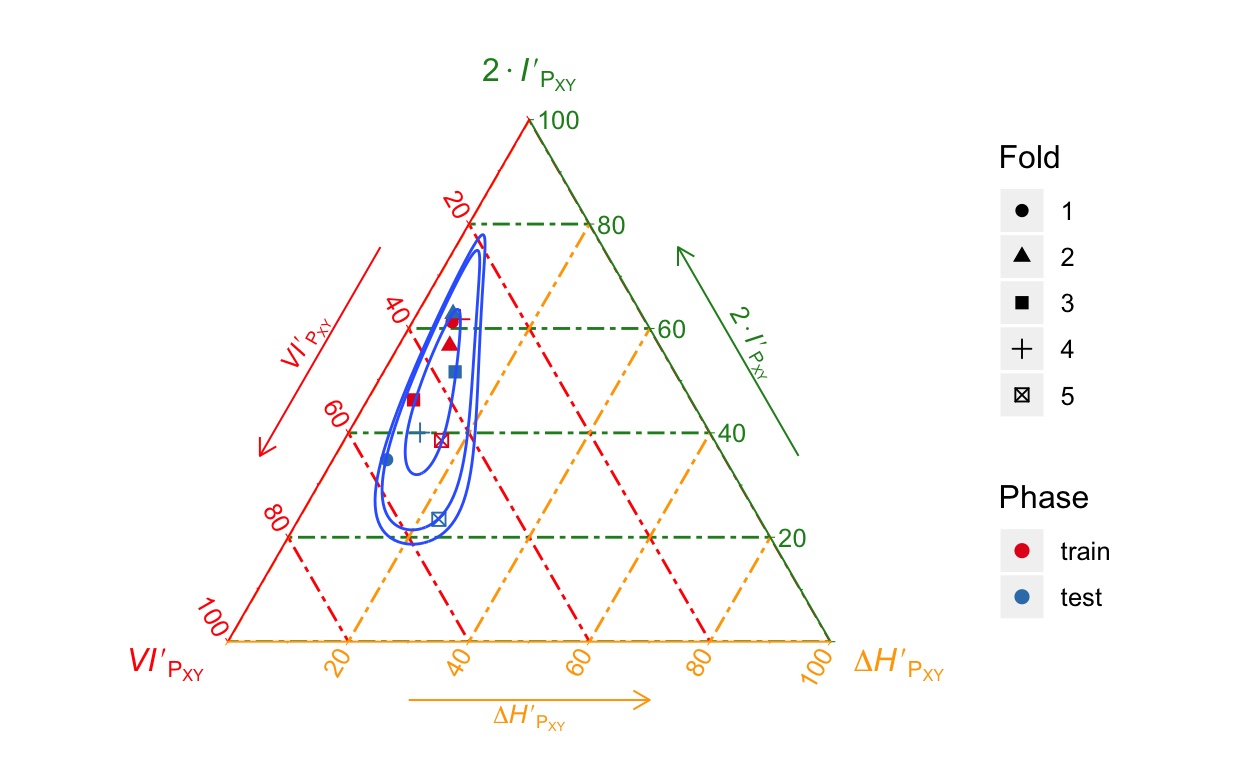
\includegraphics[width=\linewidth]{Figuras_tfg/ET_Iono_PCA_Mlp_Confidence}
	\caption{Entropy Triangle confidence interval using PCA + Mlp in Ionosphere}
	\label{fig:figure_Mlp_Iono_ET_PCA_Confidence}
\end{figure}

As seen on the Iris dataset, the sparsity of our points is greater when using the MLP. This behavior is clearly recognizable in Figure \ref{fig:figure_Mlp_Iono_ET_Auto} and Figure \ref{fig:figure_Mlp_Iono_ET_PCA}. We can also see that the degradation of results when compared to the Iris dataset is noticeable. Both the PCA and the Autoencoder don't seem to outperform each other by a great margin. They do seem to improve the outcome of the predictions from the Knn, but the unbalancing of the dataset is affecting its performance. \par

\subsection{Results discussion}

If we want to further analyze the best classifier + transformation we must once again plot the total testing fold coordinates:

\begin{figure}[H]
	\centering
	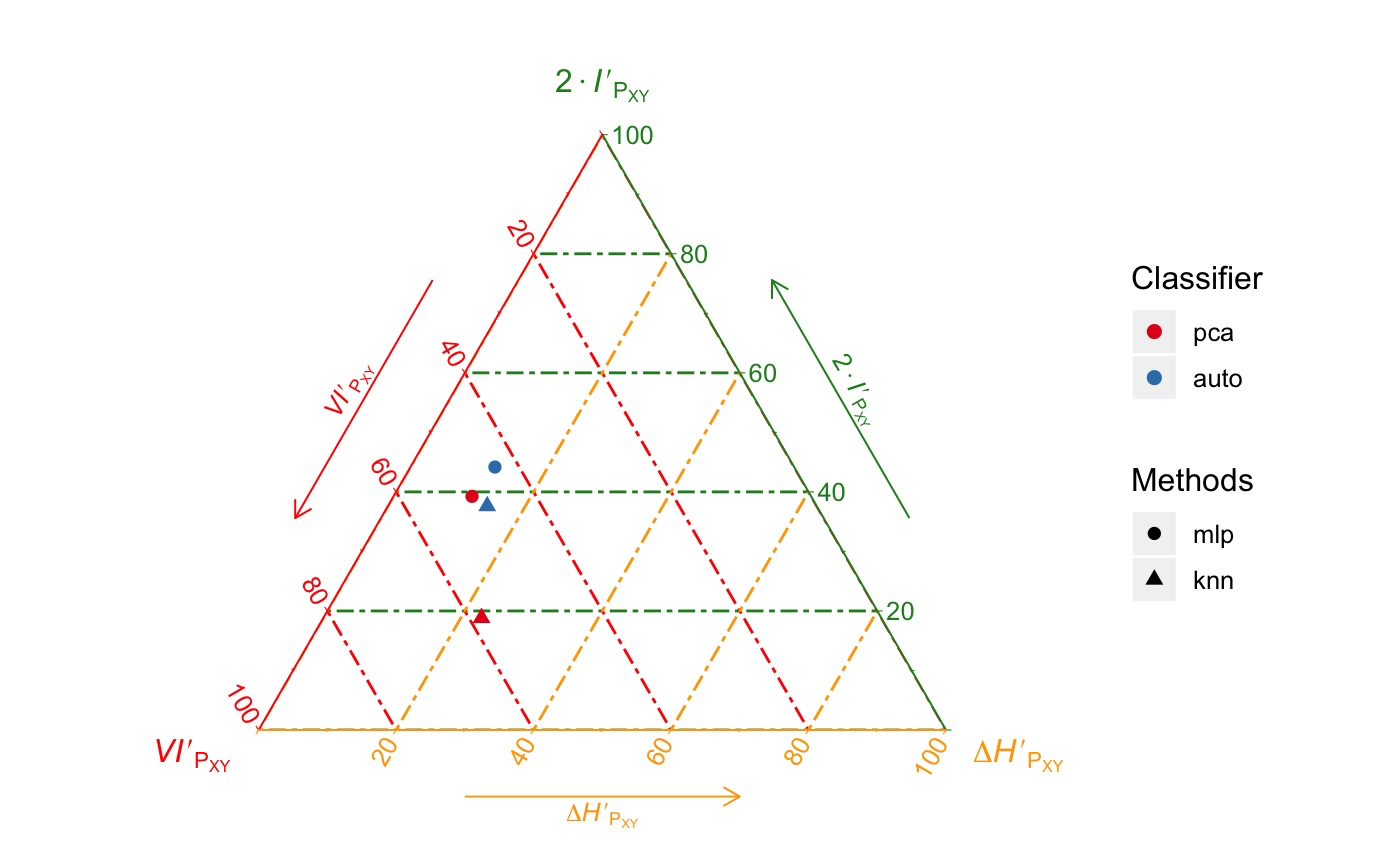
\includegraphics[width=1\linewidth]{Figuras_tfg/ET_Iono_Total_Results}
	\caption{Entropy Triangle in Ionosphere with the total test fold value}
	\label{fig:figure_Total_Ionosphere_ET}
\end{figure}

In Ionosphere, Figure \ref{fig:figure_Total_Ionosphere_ET} shows that the Autoencoder is more reliable to classify Ionosphere as both the MLP and the Knn seem to be close to each other in the ET, while the differences in the PCA are 
too great to consider that the Knn can be used to classify Ionosphere.\par

In the particular case of Ionosphere, it is interesting to take a look at the confusion matrices from the folds, as well as the accuracy of the training. We can also use some of the data acquired from the training of Iris to compare them. \par

For example, we can compare the third fold from the MLP in the Autoencoder from  Iris and in Ionosphere we are taking the first fold from the MLP in the PCA:

\begin{table}[H]
	\label{tab:Iris_vs_Ionosphere}
	\caption{Comparison of Iris and Ionosphere confusion matrices}
	\begin{tabular}{@{}cc@{}}
	\begin{minipage}{.5\linewidth}
		\subcaption{Iris confusion matrix}
		\centering
\begin{tabular}{|p{1cm}|p{1cm}|p{1cm}|} % <-- Alignments: 1st column left, 2nd middle and 3rd right, with vertical lines in between
	\multicolumn{3}{c}{Accuracy = 93 \%} \\
	\hline
	
	10 &  0 & 0 \\ \hline
	 0 & 10 & 0 \\ \hline
	 0 &  9 & 10\\
	 \hline
\end{tabular}
    
	\end{minipage}%
	\begin{minipage}{.5\linewidth}
	\subcaption{Ionosphere confusion matrix}
		\centering
		
	\begin{tabular}{|p{1cm}|p{1cm}|} % <-- Alignments: 1st column left, 2nd middle and 3rd right, with vertical lines in between
		\multicolumn{2}{c}{Accuracy = 94 \%} \\
		\hline
		
		18 &  3 \\ \hline
	 	7  & 42 \\
		
		\hline
	\end{tabular}
	
	\end{minipage} 
\end{tabular}
\end{table}

From analyzing Table \ref{tab:Iris_vs_Ionosphere}, we get more or less the same accuracies on both instances of the folds, but only in case of the Iris MLP we are getting results with that level of certainty. The Ionosphere dataset is so unbalanced and that its observations, regardless of the level of accuracy shown, are forcing errors on our predictor. This is an example of the \textbf{accuracy paradox} mentioned on \autoref{chap:TheorethicalBackground}.

\section{MNIST Dataset}
\subsection{Data Preparation}

All the necessary processes needed to transform our data into a valuable representation of it for the purpose of the Bachelor Thesis have been explained on Section \ref{subsec:MNIST}.

\subsection{The Autoencoder}
The Autoencoder used for the MNIST dataset has the most complex structure in terms of computational power out of all of the considered implementations for the sake of this thesis. 

\begin{table}[H]
	\caption{MNIST Autoencoder layers of the encoder.}
	\begin{center}
		\label{tab:table_MNIST_auto_encoder}
		\begin{tabular}{c|c|c} % <-- Alignments: 1st column left, 2nd middle and 3rd right, with vertical lines in between
			\textbf{Number of Layers} & \textbf{Size} & \textbf{Activation Function} \\
			\hline
			First & 784 & None\\
			Second & 1000 & Relu\\
			Third & 500  & Relu\\
			Fourth & 250 & Relu\\
			Fifth or Middle & 64 & Relu\\
		\end{tabular}
	\end{center}
\end{table}

\begin{table}[H]
	\caption{MNIST layers of the decoder.}
	\begin{center}
		\label{tab:table_MNIST_auto_decoder}
		\begin{tabular}{c|c|c} % <-- Alignments: 1st column left, 2nd middle and 3rd right, with vertical lines in between
			\textbf{Number of Layers} & \textbf{Size} & \textbf{Activation Function} \\
			\hline
			First or Middle & 64 & None\\
			Second & 250 & Relu\\
			Third & 500  & Relu\\
			Fourth & 1000 & Relu\\
			Fifth & 784 & Sigmoid \\
		\end{tabular}
	\end{center}
\end{table}

The Autocoder has a large amount of observations (Around 287.1 megabits only for the $X$ training component), so we expect the training time to be longer than the previous datasets. We are also going to keep the same configuration for the activation functions of the architecture, as the other Autoencoders  have proven successful to the transference of information.

\subsection{MLP on PCA and Autoencoder}

The structure implemented for the MLP in the Autoencoder and in the PCA will be completely different. As seen in both Table \ref{tab:table_MNIST_auto_encoder} and Table \ref{tab:table_MNIST_auto_decoder}, the size of our variables is 64 in the $\hat{Z}$ from the Autoencoder, but the PCA creates a matrix with the same measures as the input $\hat{X}$, which makes us have to increase the size of our MLP greatly, thus making us add an extra layer to improve it's performance.
\par	

\begin{table}[H]
	\caption{MNIST MLP layers of the Autoencoder}
	\begin{center}
		\label{tab:table_MNIST_MLP_auto}
		\begin{tabular}{c|c|c} % <-- Alignments: 1st column left, 2nd middle and 3rd right, with vertical lines in between
			\textbf{Number of Layers} & \textbf{Size} & \textbf{Activation Function} \\
			\hline
			First & 64 & None\\
			Second & 128 & Relu\\
			Third & 64  & Sigmoid\\
			Fourth & 10 & Softmax\\
		\end{tabular}
	\end{center}
\end{table}

\begin{table}[H]
	\caption{MNIST MLP layers of the PCA}
	\begin{center}
		\label{tab:table_MNIST_MLP_pca}
		\begin{tabular}{c|c|c} % <-- Alignments: 1st column left, 2nd middle and 3rd right, with vertical lines in between
			\textbf{Number of Layers} & \textbf{Size} & \textbf{Activation Function} \\
			\hline
			First & 1000 & None\\
			Second & 500 & Relu\\
			Third & 125  & Relu\\
			Fourth & 64 & Sigmoid\\
			Fifth & 10 & Softmax \\
		\end{tabular}
	\end{center}
\end{table}

As we can see on Table \ref{tab:table_MNIST_MLP_pca} the PCA MLP has the advantage of being composed by a greater amount of neurons, making it more computationally powerful and thus having an advantage towards the smaller Autoencoder MLP. 


\begin{figure}[H]
	\centering
	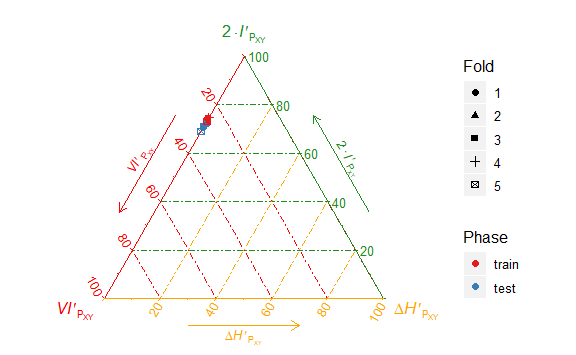
\includegraphics[width=1\linewidth]{Figuras_tfg/MNIST_Autoencoder_mlp}
	\caption{Entropy Triangle using Autoencoder + Mlp in MNIST}
	\label{fig:figure_Mlp_MNIST_ET_Auto}
\end{figure}

\begin{figure}[H]
	\centering
	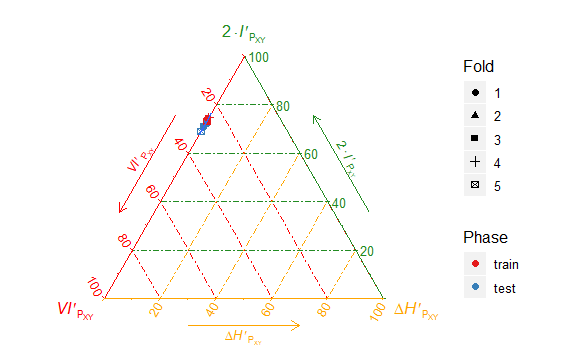
\includegraphics[width=1\linewidth]{Figuras_tfg/MNIST_Autoencoder_mlp_Confidence}
	\caption{Entropy Triangle confidence interval using Autoencoder + Mlp in MNIST}
    \label{fig:figure_Mlp_MNIST_ET_Auto_Confidence}
\end{figure}

\begin{figure}[H]
	\centering
	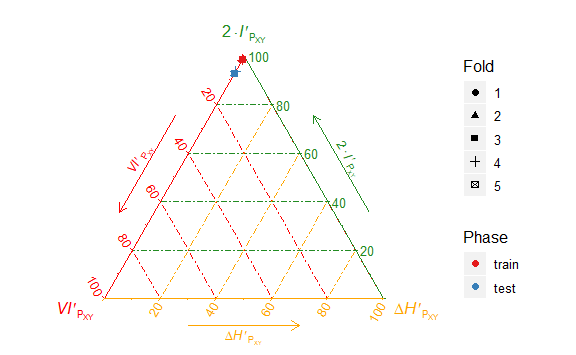
\includegraphics[width=1\linewidth]{Figuras_tfg/MNIST_PCA_mlp}
	\caption{Entropy Triangle using PCA + Mlp in MNIST}
	\label{fig:figure_Mlp_MNIST_ET_PCA}
\end{figure}

\begin{figure}[H]
	\centering
	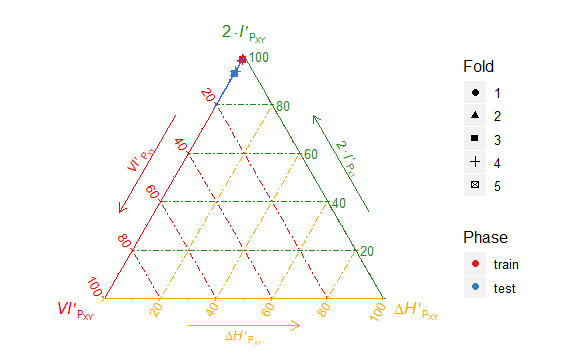
\includegraphics[width=1\linewidth]{Figuras_tfg/MNIST_PCA_mlp_Confidence}
	\caption{Entropy Triangle confidence interval using PCA + Mlp in MNIST}
	\label{fig:figure_Mlp_MNIST_ET_PCA_Confidence}
\end{figure}

After plotting both Figure \ref{fig:figure_Mlp_MNIST_ET_Auto} and Figure \ref{fig:figure_Mlp_MNIST_ET_PCA} we can clearly see that the PCA has proven to be the best choice to classify MNIST. Its training folds have placed in the tip of the ET, and although the test folds have performed worst than them, they are still placed highly. On the other hand, the MLP classifier on the Autoencoder has good informational characteristic, but it lacks the predictive power of the PCA.\par

The Figures representing the confidence intervals in this dataset don't provide a lot of information about them. Practically both of them are moving along the $VI'_{P_{XY}}$ line, but regarding delta of the entropies to be constant and the Mutual Information as variable.\par

\subsection{Results discussion} 

\begin{figure}[H]
	\centering
	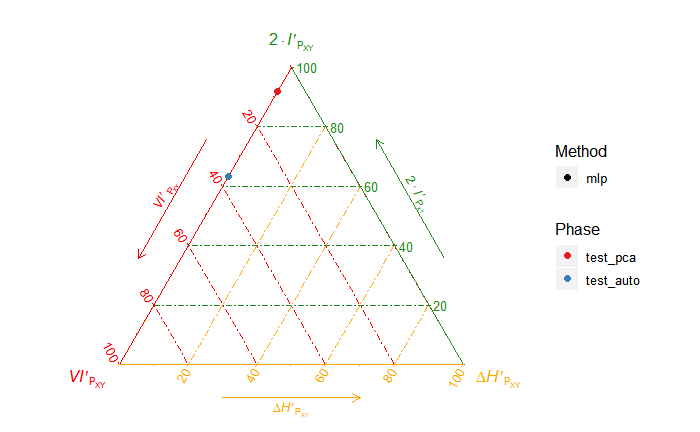
\includegraphics[width=1\linewidth]{Figuras_tfg/MNIST_performance_test}
	\caption{Entropy Triangle in MNIST with the total test fold value}
	\label{fig:figure_Total_MNIST_ET}
\end{figure}

By looking at Figure \ref{fig:figure_Total_MNIST_ET} it is confirmed that our previous affirmations about MNIST were correct. The PCA has outperformed the Autoencoder and the test fold has placed the highest out of all the experiment performed in this Bachelor Thesis. \par

We knew from our investigation before the experiments that great results on the classification of MNIST had been achieved throughout the years, and it has proven to be the most reliable source for the prediction of values to us. It can be due to the fact that it has the greatest number of observations, and despite of its size it can allow for structures such as the MLP to get plenty of data to be trained with and thus get better results at predicting the test folds. \par


